\section{Problem Set 3}
\subsection{We are Close in Near-Circular Orbits}

\subsubsection{Initial Conditions for HCW}

We would like to use the Hill-Clohessy-Wiltshire (HCW) equations to give us a clear solution to the relative motion of the deputy satellites. However, the HCW equations assume that the motion of the deputy with respect to the chief is very small compared to the orbit radius, as they rely on linearizing the non-linear equations of motion the initial conditions for this are built over the original absolute and relative initial conditions for SV1, SV2, and SV3 that were previous defined in Table \ref{tab:abs_oe} and Table \ref{tab:relative_oe}.

The eccentricity of SV1 is already very low, as seen in Table \ref{tab:abs_oe_kepler} (and meets the conditions for applying HCW). Therefore, the orbital elements of the chief did not need to be modified. However, the relative orbital elements initial conditions create a large separation between SV1 and SV2/SV3. So the quasi-nonsingular relative orbital elements are modified to be as in Table \ref{tab:relative_oe_hcw} below. These are written in order as described in Equation \ref{eq:quasi_nonsign_roe}.

\begin{table}[h!]
\centering
\begin{tabular}{ll}
\toprule
\textbf{ID} & \textbf{HCW Conditions} \\
\midrule
SV2 & $\delta\boldsymbol{\alpha} = [0, 0, 0, 300, 0, 300]~\text{m}$ \\
SV3 & $\delta\boldsymbol{\alpha} = [0, 0, 0, 250, 0, -250]~\text{m}$ \\
\bottomrule
\end{tabular}
\caption{Quasi-Nonsingular Relative Orbit Parameters for SV2 and Sv3 to apply for HCW}
\label{tab:relative_oe_hcw}
\end{table}

The main differences in these quasi-nonsingular relative orbital elements (and the justification for these changes), are:
\begin{itemize}
    \item $\delta\alpha$ is 0 for both SV2 and SV3, so that they have the same semi-major axes as SV1.
    \item The $\delta\lambda$ for both deputy satellites is reduced to 0. This helps reduce the separation between the deputies and the chief
    \item $\delta e_x$and $\delta i_x$ are set to zero for convenience, and to easily create a $\boldsymbol{e}-\boldsymbol{i}$ vector angle separation of $0^\circ$.
    \item $\delta e_y$ and $\delta i_y$ are set to convenient values close to the original relative orbital elements in Table \ref{tab:relative_oe}.
\end{itemize}

Based on these initial conditions, we see that the ratio of the maximum separation between spacecraft is small relative to the distance of the chief from the primary attractor. This is verified by propagating the nonlinear equations of motion throughout the time scale to get the position of the chief and the relative positions of the deputies, and finding the average ratio over time (since the orbit is circular, this worst-case ratio is very close to the average). We see that the average ratios are

\begin{align}
    \frac{\rho_{SV2}}{r_{SV1}} = 7.25\cdot10^{-5} \\
    \frac{\rho_{SV3}}{r_{SV1}} = 6.04\cdot10^{-5}
\end{align}
Both of these are well below the $10^{-3}$ requirement.

\subsubsection{Transforming the Initial Conditions} \label{sec:hcw_initial_conditions}
We can convert the initial conditions set in Table \ref{tab:relative_oe_hcw} to different representations. The initial conditions for the chief are not recalculated, as these have not been modified from previous sections.

\textbf{ECI and Absolute Orbital Elements} \\
Using the transformations highlighted in Equation \ref{eq:quasi_nonsign_roe}, 
we convert the quasi-nonsingular relative orbital elements into absolute orbital elements. The results for SV2 and SV3 are given in Table \ref{tab:abs_oe_kepler_SV2_HCW} and Table \ref{tab:abs_oe_kepler_SV3_HCW}. The absolute orbital elements of the chief remain the same as in Table \ref{tab:abs_oe_kepler}.

\begin{table}[h]
\centering
\begin{tabular}{cccccc} \hline
    $a$ & $e$ & $i$ & $\omega$ & $\Omega$ & $\nu$ \\ \hline 
     6944 km & 0.0016 & 99.4 $^\circ$ & 91.3946$^\circ$ & -151.10$^\circ$ & -139.417$^\circ$ \\ \hline
\end{tabular}
\caption{Initial Keplerian Orbit Parameters of SV2, modified for applying HCW}
\label{tab:abs_oe_kepler_SV2_HCW}
\end{table}

\begin{table}[h]
\centering
\begin{tabular}{cccccc} \hline
    $a$ & $e$ & $i$ & $\omega$ & $\Omega$ & $\nu$ \\ \hline 
     6944 km & 0.0016 & 99.4 $^\circ$ & 91.4003$^\circ$ & -151.10$^\circ$ & -139.423$^\circ$ \\ \hline
\end{tabular}
\caption{Initial Keplerian Orbit Parameters of SV3, modified for applying HCW}
\label{tab:abs_oe_kepler_SV3_HCW}
\end{table}

These Keplerian orbital elements are then converted to ECI co-ordinates using the expressions provided in Section \ref{sec:initial_ECI}. The initial ECI co-ordinates of the chief remain the same as in Equation \ref{eq:SV1_initial_ECI}. Equations \ref{eq:SV2_HCW1_ECI_initial} and \ref{eq:SV3_HCW1_ECI_initial} provide the ECI co-ordinates of SV2 and SV3. 
\begin{align} \label{eq:SV2_HCW1_ECI_initial}
    r_{0, ECI, SV2} &= \begin{bmatrix}
        -3664.4 \\
        -2988.6 \\
        -5102.7
    \end{bmatrix} km \\
    v_{0, ECI, SV2} &= \begin{bmatrix}
        -5.3182 \\
        -1.9926 \\
        4.9928
    \end{bmatrix} \frac{km}{s}
\end{align}

[-3.664634040411143e+03;-2.988364002505523e+03;-5.102717495801277e+03;-5.318448889943923;-1.992230030548635;4.992735637485701]
\begin{align} \label{eq:SV3_HCW1_ECI_initial}
    r_{0, ECI. SV3} &= \begin{bmatrix}
        -3664.6 \\
        -2988.4 \\
        -5102.7
    \end{bmatrix} km \\
    v_{0, ECI, SV3} &= \begin{bmatrix}
        -5.3184 \\
        -1.9922 \\
        4.9927
    \end{bmatrix} \frac{km}{s}
\end{align}
\textbf{Relative Position and Velocity in Chief's RTN frame, Orbital Element Differences} \\
Since the initial conditions of SV1, SV2, and SV3 are known, we can find the positions and velocities of SV2 and SV3 in SV1's RTN frame using the equations highlighted in Section \ref{sec:nonlinear_rel_eom}. These are provided below in Equations \ref{eq:SV2_HCW_RTN_init} and \ref{eq:SV3_HCW_RTN_init}.

\begin{align} \label{eq:SV2_HCW_RTN_init}
    r_{0, RTN. SV2} &= \begin{bmatrix}
        0.3256 \\
        -0.4989 \\
        -0.5971
    \end{bmatrix} km \\
    v_{0, RTN, SV2} &= \begin{bmatrix}
        -2.0102 \\
        -5.8056 \\
        -7.7372
    \end{bmatrix}\cdot 10^{-4} \frac{km}{s}
\end{align}

\begin{align} \label{eq:SV3_HCW_RTN_init}
    r_{0, RTN. SV2} &= \begin{bmatrix}
        0.2433 \\
        -0.3730 \\
        -0.4914
    \end{bmatrix} km \\
    v_{0, RTN, SV2} &= \begin{bmatrix}
        -1.5210 \\
        -4.3352 \\
        -6.3669
    \end{bmatrix}\cdot 10^{-4} \frac{km}{s}
\end{align}

The differences in the initial orbital elements between the chief and the deputies is best conveyed by the quasi-nonsingular relative orbital elements that are provided in Table \ref{tab:relative_oe_hcw}.

\subsubsection{Computing the Integration Constants}

The Hill-Clohessy Wiltshire equations for linearized relative orbital dynamics allows for analytical solutions of the RTN position $[x, y, z]^\top$ and the RTN velocity $[\dot{x}, \dot{y}, \dot{z}]^\top$ of the deputy satellites in the chief's RTN frame. This solution can be expressed as a function of time, when six integration constants are known (one for each state). The integration constants and the satellite's RTN state are related the Matrix-Vector solution for HCW, given in Equation \ref{eq:HCW_solution}, 


\begin{align} \label{eq:HCW_solution}
\begin{bmatrix}
x \\ y \\ z \\ \dot{x} \\ \dot{y} \\ \dot{z}
\end{bmatrix}
&=
\begin{bmatrix}
a I_{3 \times 3} & 0_{3 \times 3} \\
0_{3 \times 3} & a n I_{3 \times 3}
\end{bmatrix}
\begin{bmatrix}
1 & \sin nt & \cos nt & 0 & 0 & 0 \\
-\frac{3}{2}nt & 2 \cos nt & -2 \sin nt & 1 & 0 & 0 \\
0 & 0 & 0 & 0 & \sin nt & \cos nt \\
0 & \cos nt & -\sin nt & 0 & 0 & 0 \\
-\frac{3}{2} & -2 \sin nt & -2 \cos nt & 0 & 0 & 0 \\
0 & 0 & 0 & 0 & \cos nt & -\sin nt
\end{bmatrix}
\begin{bmatrix}
K_1 \\ K_2 \\ K_3 \\ K_4 \\ K_5 \\ K_6
\end{bmatrix},
\end{align}

where $a$ represents the semi-major axis, $n$ represents the mean motion, and $t$ is time since the initial conditions. $K_1$ through $K_6$ are the integration constants. The matrix relating the integration constants and the state, when the state is made of integration constants (e.g., with ROE), is called the State Transition Matrix (STM). The STM maps the state at a certain time to the state at a future time. 

To calculate the integration constants, $t = 0$ in the STM, and the state is set to the initial conditions calculated in Section \ref{sec:hcw_initial_conditions}. Then the inverse of the STM matrix is taken to find the state.

\begin{align}
    \begin{bmatrix}
K_1 \\ K_2 \\ K_3 \\ K_4 \\ K_5 \\ K_6
\end{bmatrix} = \left(\begin{bmatrix}
a I_{3 \times 3} & 0_{3 \times 3} \\
0_{3 \times 3} & a n I_{3 \times 3}
\end{bmatrix}
\begin{bmatrix}
1 & 0 & 1 & 0 & 0 & 0 \\
0 & 2 & 0 & 1 & 0 & 0 \\
0 & 0 & 0 & 0 & 0 & 1 \\
0 & 1 & 0 & 0 & 0 & 0 \\
-\frac{3}{2} & 0 & -2 & 0 & 0 & 0 \\
0 & 0 & 0 & 0 & 1 & 0
\end{bmatrix}\right)^{-1} \begin{bmatrix}
x_0 \\ y_0 \\ z_0 \\ \dot{x}_0 \\ \dot{y}_0 \\ \dot{z}_0
\end{bmatrix}
\end{align}

For our chosen initial conditions, the integration constants computed are provided in Table \ref{tab:integration_constants_HCW}.

\begin{table}[ht]
    \centering
    \renewcommand{\arraystretch}{1.2}
    \begin{tabular}{c c c}
        \toprule
        \textbf{Constant} & \textbf{SV2} & \textbf{SV3} \\
        \midrule
        $K_1$ & $3.796\cdot10^{-7}$ & $3.172\cdot10^{-7}$ \\
        $K_2$ & $-2.880\cdot10^{-5}$ & $-2.398\cdot10^{-5}$ \\
        $K_3$ & $3.173\cdot10^{-5}$& $2.645\cdot10^{-5}$\\
        $K_4$ & $-2.100\cdot10^{-7}$ & $-1.757\cdot10^{-7}$ \\
        $K_5$ & $-3.204\cdot10^{-5}$ & $2.670\cdot10^{-5}$ \\
        $K_6$ & $-2.895\cdot10^{-5}$ & $2.4123\cdot10^{-5}$ \\
        \bottomrule
    \end{tabular}
    \caption{Integration Constants for SV2 and SV3 Used in HCW Analytical Solution}
    \label{tab:integration_constants_HCW}
\end{table}

\subsubsection{Relative State Propagation Using HCW Solution}

With the integration constants known, we can find the state (position and velocity) of SV2 and SV3 over all the 15 orbits we want to simulate, using the relation in Equation \ref{eq:HCW_solution}. Since this assumes circular orbits, we can use time as our independent variable rather than true anomaly. The time series used is the same Equation \ref{eq:timestep}, except with 15 orbits instead of 25. This is done for both SV2 and SV3.

Figures \ref{fig:hcw_sv2_pos_vel} and \ref{fig:hcw_sv2_pos_vel} showcase the position and velocity of SV2 and SV3 over time with HCW. Figure \ref{fig:hcw_projections} projects the RTN projection of SV2 and SV3 on the R-N, R-T, and T-N frames to give a better idea of the relative motion of the deputy satellites. Figure \ref{fig:hcw_comparisons_projections} compares the HCW result with the Fundamental Equations of Relative Motion (FERM) result, computed with the nonlinear equations described in Section \ref{sec:nonlinear_rel_eom}. Finally, for additional visualization, Figure \ref{fig:hcw_3d_side_by_side} showcases the trajectory of SV2 and SV3 in the chief's RTN frame over time in 3D.

The results in these plots are analyzed in the Section \ref{sec:analysis_of_hcw}.

\begin{figure}[htpb]
    \centering
    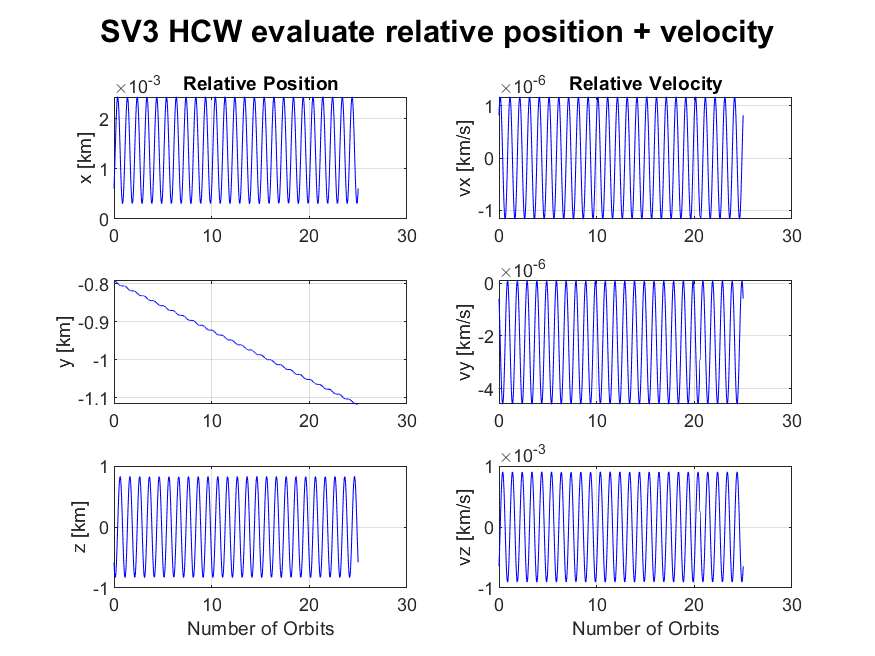
\includegraphics[width=0.7\linewidth]{sim/figures/PS3/HCW_pos_vel_SV2.png}
    \caption{Relative position and velocity of SV2 in the chief's RTN frame, evaluated using HCW equations.}
    \label{fig:hcw_sv2_pos_vel}
\end{figure}

\begin{figure}[htpb]
    \centering
    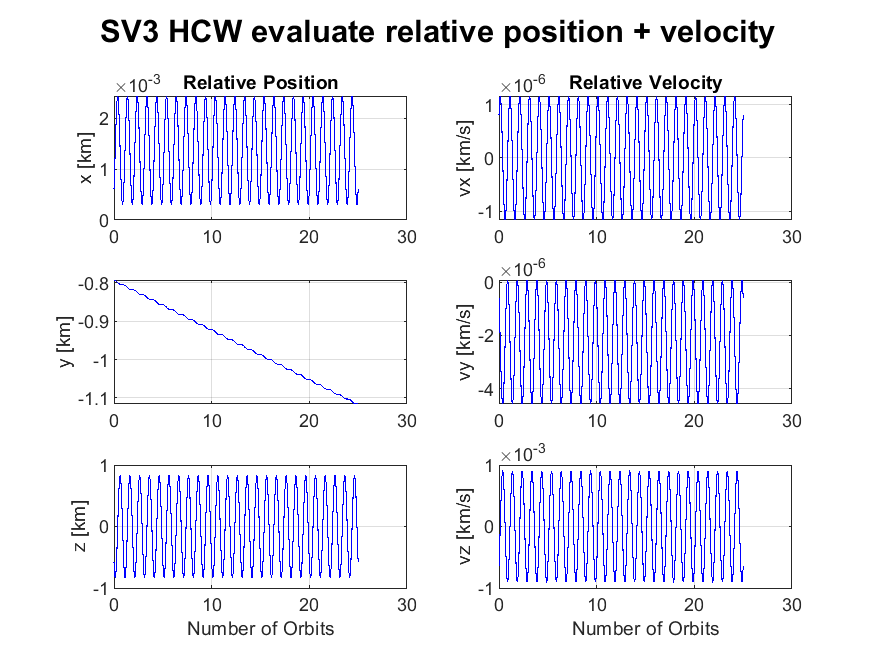
\includegraphics[width=0.7\linewidth]{sim/figures/PS3/HCW_pos_vel_SV3.png}
    \caption{Relative position and velocity of SV3 in the chief's RTN frame, evaluated using HCW equations.}
    \label{fig:hcw_sv2_pos_vel}
\end{figure}

\begin{figure}[htpb]
    \centering
    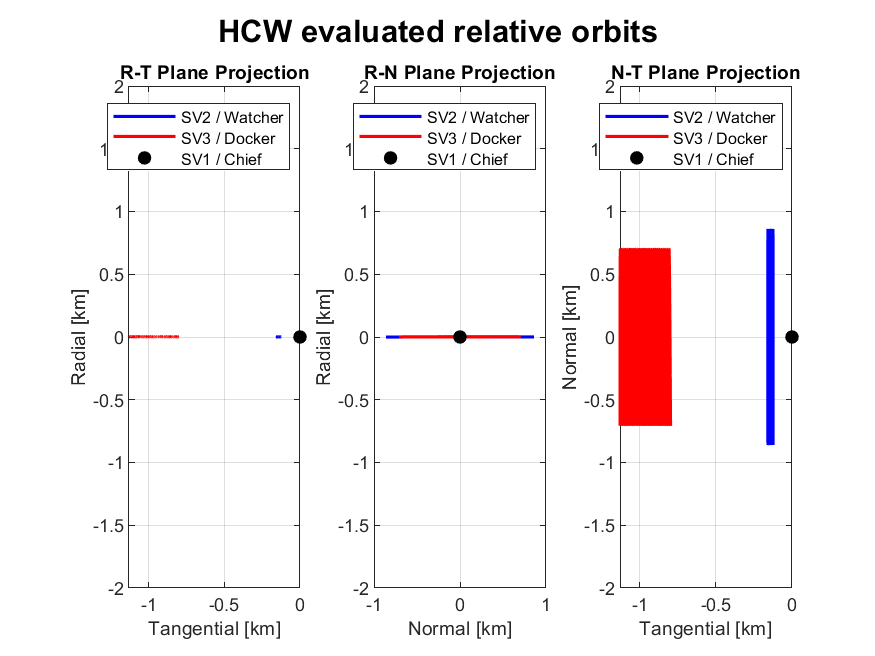
\includegraphics[width=0.7\linewidth]{sim/figures/PS3/RTN_projections_HCW.png}
    \caption{RTN Projections of SV2 and SV3 trajectories calculating using HCW}
    \label{fig:hcw_projections}
\end{figure}

\begin{figure}[htpb]
    \centering
    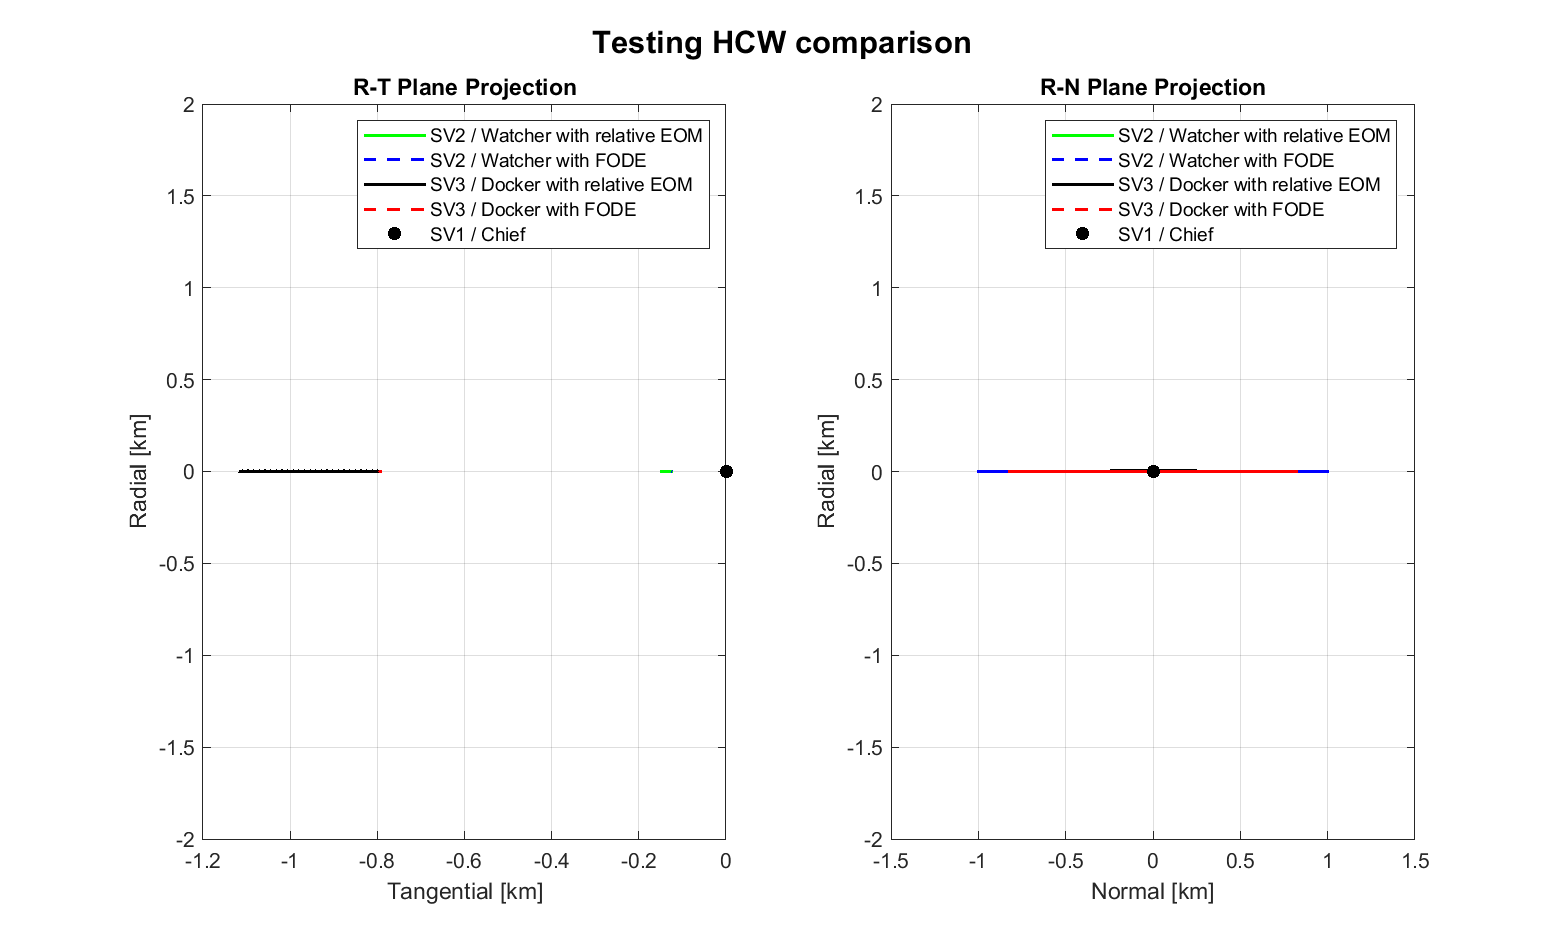
\includegraphics[width=0.75\linewidth]{sim/figures/PS3/RTN_projections_HCW_comparison.png}
    \caption{RTN Projections of SV2 and SV3 comparison between HCW and FERM.}
    \label{fig:hcw_comparisons_projections}
\end{figure}

\begin{figure}[htpb]
    \centering
    \begin{subfigure}[t]{0.45\linewidth}
        \centering
        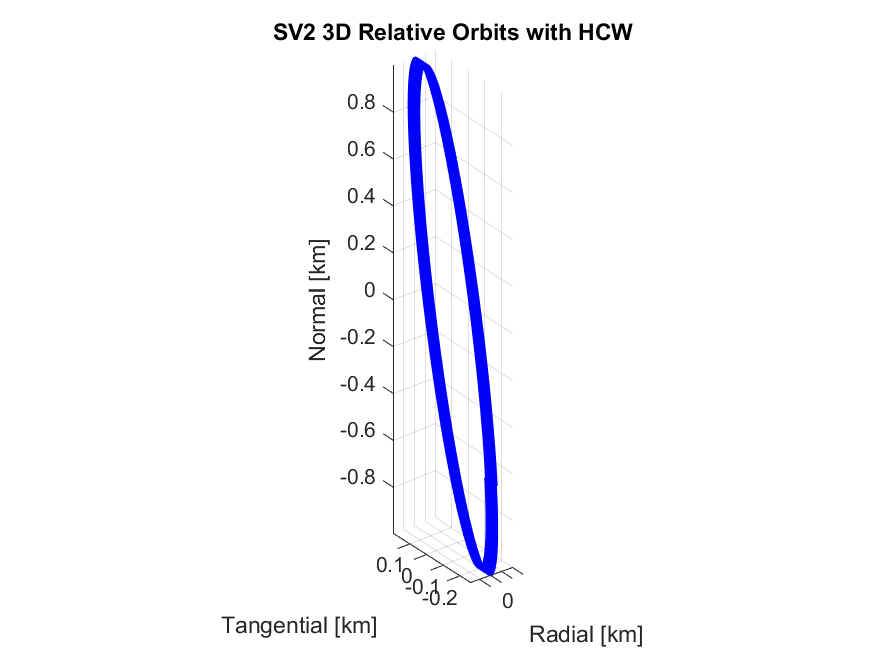
\includegraphics[width=1.2\linewidth]{sim/figures/PS3/3D_HCW_orbit_SV2.png}
        \caption{SV2-HCW Orbit}
        \label{fig:hcw_sv2}
    \end{subfigure}%
    \begin{subfigure}[t]{0.45\linewidth}
        \centering
        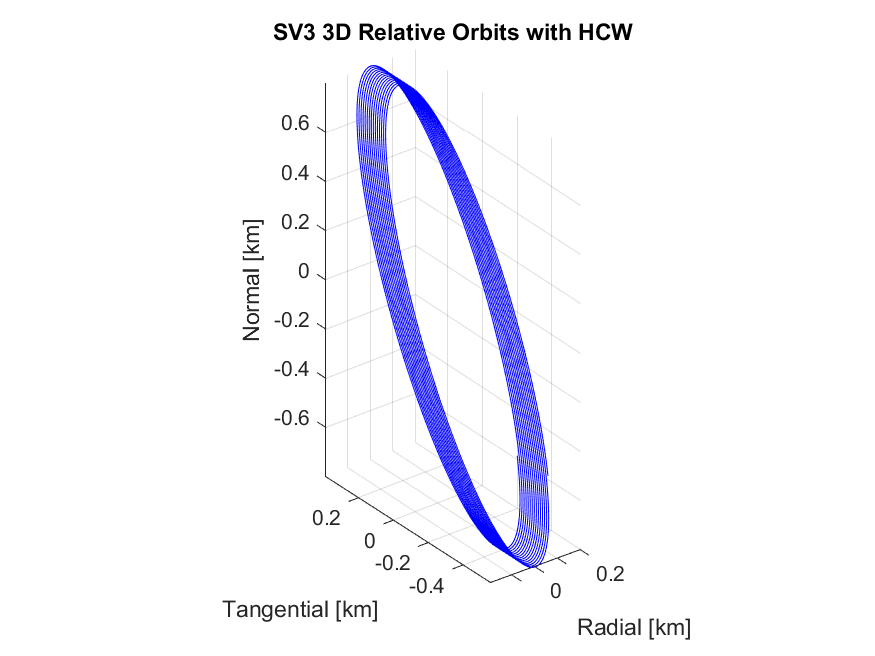
\includegraphics[width=1.2\linewidth]{sim/figures/PS3/3D_HCW_orbit_SV3.png}
        \caption{SV3-HCW Orbit}
        \label{fig:hcw_sv3}
    \end{subfigure}
    \caption{3D HCW-relative orbits of SV2 and SV3.}
    \label{fig:hcw_3d_side_by_side}
\end{figure}

\subsubsection{Analysis of HCW Solution Behavior}\label{sec:analysis_of_hcw}
Analyzing Figures \ref{fig:hcw_sv2_pos_vel}
to \ref{fig:hcw_3d_side_by_side}, there are a few common trends that we can observe:
\begin{enumerate}
    \item There is a drift in the along-track position. This drift is seen only in the HCW solution and is not present in the result from propagating the fundamental non-linear equations of motion.
    \item The projection of the orbit in the R-T and R-N planes is elliptical (ignoring the drift in the along-track direction).
\end{enumerate}

First, we address the elliptical orbit's shape and orientation. This elliptical orbit can be related to the relative eccentricity vector $\boldsymbol{\delta e} = [\delta e_x, \delta e_y]^\top$ and the relative inclination vector $\boldsymbol{\delta i} = [\delta i_x, \delta i_y]^\top$. With the selected initial conditions in Table \ref{tab:relative_oe_hcw}, we see that the angle between $\boldsymbol{\delta e}$ and $\boldsymbol{\delta i}$ is $0$, as they both lie along the y-axis. The two vectors being parallel results in an elliptical relative orbit around the chief that is safe and avoids collision even under uncertainty in the along track direction (see Figure \ref{fig:relative_orbit_geometry}).

\begin{figure}[htpb]
    \centering
    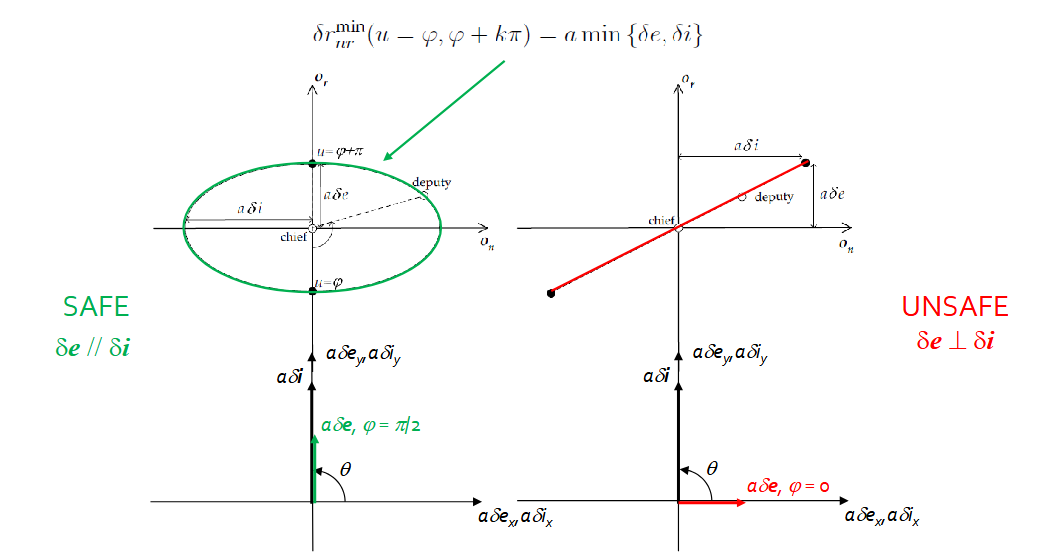
\includegraphics[width=0.75\linewidth]{LaTeX//PS3/relative_orbit_geometry.png}
    \caption{Based one the angle between the relative inclination vector and the relative eccentricity vector, the relative orbit can be either an ellipse or a line passing through the chief. By choosing parallel vectors we create a safe ellipse.}
    \label{fig:relative_orbit_geometry}
\end{figure}

The integration constants provided in Table \ref{tab:integration_constants_HCW} also provide insight into the shape and position of the elliptical orbit relative to the chief. Figure \ref{fig:hcw_gemeotry} provides this relation. 

\begin{figure}[htpb]
    \centering
    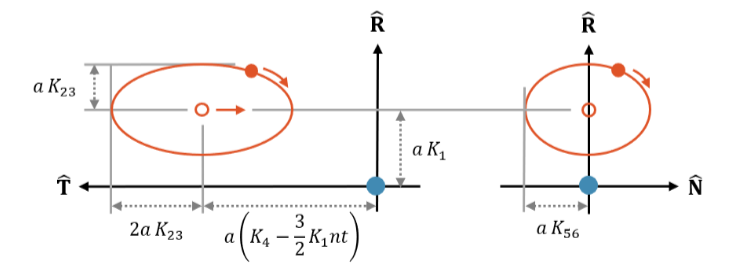
\includegraphics[width=0.75\linewidth]{LaTeX//PS3/hcw_integration_constants.png}
    \caption{Geometric Significance of the HCW integration constants. Here, $K_{23} = \sqrt{K_2^2 + K_3^2}$ \cite{willis2023analytical}}
    \label{fig:hcw_gemeotry}
\end{figure}

If we compute these quantities for SV2 and SV3, we get the results in Table \ref{tab:HCW_geometry_values}. Using these values in the Figure \ref{fig:hcw_gemeotry} guide, we see that our integration constants correspond correctly to the geometry we see in Figure \ref{fig:hcw_projections}.

\begin{table}[htpb]
    \centering
    \renewcommand{\arraystretch}{1.2}
    \begin{tabular}{c c c}
        \toprule
        \textbf{Value (in km)} & \textbf{SV2} & \textbf{SV3} \\
        \midrule
        $2aK_{23}$ & 0.595 & 0.496 \\
        $aK_{56}$ & 0.300 & 0.250 \\
        $aK_1$ & $2.64\cdot10^{-3}$& $2.20\cdot10^{-3}$\\
        \bottomrule
    \end{tabular}
    \caption{Values derived from the HCW geometry equations that correspond to the ellipse shape as seen in Figure \ref{fig:hcw_gemeotry}.}
    \label{tab:HCW_geometry_values}
\end{table}

An interesting fact is that these correspond very well with the relative orbital elements chosen in Table \ref{tab:relative_oe_hcw}!

We also see that there is a slow drift in the along-track component in the HCW formulation, which means that we are seeing unbounded motion. This is because there is an unstable mode in the HCW equations that makes the motions unstable, even if the true motion (found from using non-linear equation propagation) is bounded with $\delta a  =0$. This arises from a non-zero $K_1$ value. As seen in Table \ref{tab:HCW_geometry_values}, this value is very small but non-zero, which leads to drift. To mitigate this, initial conditions can be modified to meet the stability condition
\begin{align}
    \dot{y}_0 = -2nx_0
\end{align}
This stability condition ensures that the first-order relative motion (which is all that HCW captures) remains bounded, preventing the drift in the along-track motion. Having this condition also reduces $K_1 \rightarrow 0$, which would meet the dependence on $t$ in the geometry conditions of Figure \ref{fig:hcw_gemeotry}.

\newpage

\subsection{We are Close in Eccentric Orbits}
\subsubsection{Initial Conditions for Tschauner-Hempel Equations}
Now, we turn our analysis to eccentric orbits, where relative motion is described by the Tschauner-Hempel (TH) equations. The TH equations can be solved using the Yamanaka-Ankersen (YA) model. We will use the same initial conditions for the absolute and relative states as with HCW, except now the chief's orbit has an eccentricity of 0.15. The ROE for SV2 and SV3 remain the same as outlined in Table \ref{{tab:relative_oe_hcw}}, as these initial conditions also lie whtin the range of validity of the TH equations. Specifically, the chief and deputy have equal semi-major axes and the the maximum separation between spacecraft is small relative to the minimum distance from the primary attractor center. 

\subsubsection{YA Integration Constants}
From these chosen initial conditions, the 6 integration constants of the YA solution can be computed through the following process.

Willis outlines the transformation matrices ($A,B$) from YA integration constants to RTN position and velocity of the deputy \cite{willis2023analytical}. These matrices can be inverted to instead go from initial RTN position and velocity to YA integration constants. 

YA defines the following expressions:
\begin{align}
n &= \sqrt{\frac{\mu_{\text{earth}}}{a^3}} \\
\eta &= \sqrt{1 - e^2} \\
\tau &= \frac{nt}{\eta^3}\\
k &= 1 + e \cos(f) \\
k' &= -e \sin(f)
\end{align}

And the following transformation components:
\begin{align}
\psi_{x1} &= \frac{1}{k} + \frac{3}{2}k' \tau, &
\psi_{x2} &= \sin(f), &
\psi_{x3} &= \cos(f) \\
\psi_{y1} &= -\frac{3}{2}k\tau, &
\psi_{y2} &= \left(1 + \frac{1}{k}\right)\cos(f), &
\psi_{y3} &= -\left(1 + \frac{1}{k}\right)\sin(f), &
\psi_{y4} &= \frac{1}{k} \\
\psi_{z5} &= \frac{1}{k}\sin(f), &
\psi_{z6} &= \frac{1}{k}\cos(f)
\end{align}

And their respective derivatives:
\begin{align}
\psi_{x1}' &= \frac{k'}{2} - \frac{3}{2}k^2(k - 1)\tau, &
\psi_{x2}' &= k^2 \cos(f), &
\psi_{x3}' &= -k^2 \sin(f) \\
\psi_{y1}' &= -\frac{3}{2}\left(k + k^2k'\tau\right), &
\psi_{y2}' &= -(k^2 + 1)\sin(f), &
\psi_{y3}' &= -e - (k^2 + 1)\cos(f), &
\psi_{y4}' &= -k' \\
\psi_{z5}' &= e + \cos(f), &
\psi_{z6}' &= -\sin(f)
\end{align}

And finally the full transformation matrices:
\begin{align}
A &= 
\begin{bmatrix}
a\eta^2 I_{3 \times 3} & 0 \\
0 & \frac{a n}{\eta} I_{3 \times 3}
\end{bmatrix}
\end{align}

\begin{align}
B &=
\begin{bmatrix}
\psi_{x1} & \psi_{x2} & \psi_{x3} & 0 & 0 & 0 \\
\psi_{y1} & \psi_{y2} & \psi_{y3} & \psi_{y4} & 0 & 0 \\
0 & 0 & 0 & 0 & \psi_{z5} & \psi_{z6} \\
\psi_{x1}' & \psi_{x2}' & \psi_{x3}' & 0 & 0 & 0 \\
\psi_{y1}' & \psi_{y2}' & \psi_{y3}' & \psi_{y4}' & 0 & 0 \\
0 & 0 & 0 & 0 & \psi_{z5}' & \psi_{z6}'
\end{bmatrix}
\end{align}

We then invert the transformation matrices to solve for the integration constants from the initial relative position and velocity conditions:
\[
K = (A B)^{-1} \cdot \begin{bmatrix}
x_0 \\ y_0 \\ z_0 \\ \dot{x}_0 \\ \dot{y}_0 \\ \dot{z}_0
\end{bmatrix}
\]

Note that in solving this equation, $\tau$ will be zero because our initial time is 0. For our chosen initial conditions, the integration constants computed are provided in Table \ref{tab:integration_constants_HCW}.

\begin{table}[ht]
    \centering
    \renewcommand{\arraystretch}{1.2}
    \begin{tabular}{c c c}
        \toprule
        \textbf{Constant} & \textbf{SV2} & \textbf{SV3} \\
        \midrule
        $K_1$ & $0.0006\cdot10^{-4}$ & $0.0005\cdot10^{-4}$ \\
        $K_2$ & $0.0115\cdot10^{-4}$ & $-0.0090\cdot10^{-4}$ \\
        $K_3$ & $-0.4413\cdot10^{-4}$& $-0.3677\cdot10^{-4}$\\
        $K_4$ & $0.0023\cdot10^{-4}$ & $-0.0022\cdot10^{-4}$ \\
        $K_5$ & $0.4321\cdot10^{-4}$ & $-0.3600\cdot10^{-4}$ \\
        $K_6$ & $0.0004\cdot10^{-4}$ & $-0.0003\cdot10^{-4}$ \\
        \bottomrule
    \end{tabular}
    \caption{Integration Constants for SV2 and SV3 Used in YA Analytical Solution}
    \label{tab:integration_constants_YA}
\end{table}

\subsubsection{Relative State Propagation Using YA Solution}
We use the same propagation strategy as with the HCW solution, except now using the YA integration constants and STM. Specifically, we use the same $A$ and $B$ matrices described in the previous section along with the integration constants that were determined. The only difference now is that we are propagating the relative position and velocity from the integration constants by increasing time (and thus $\tau$), and first solving for the corresponding true anomaly ($f$). Then we compute the $A, B$ matrices at each time step and find the relative position and velocity using the following expression:

\[
\begin{bmatrix}
x \\ y\\ z \\ \dot{x} \\ \dot{y} \\ \dot{z}
\end{bmatrix}= (A B) \cdot K
\]

The resulting relative position and velocity 3D components of SV2 and SV3 are shown in Figures \ref{fig:YA_sol_3D_comp_SV2} and \ref{fig:YA_sol_3D_comp_SV3} respectively. Both SV2 and SV3 orbits are plotted in 3D in Figure \ref{fig:YA_sol_3D_orbits}. Finally, the RTN projections of the relative orbits are shown in Figure \ref{fig:YA_sol_RTN}.


\begin{figure}[H]
    \centering
    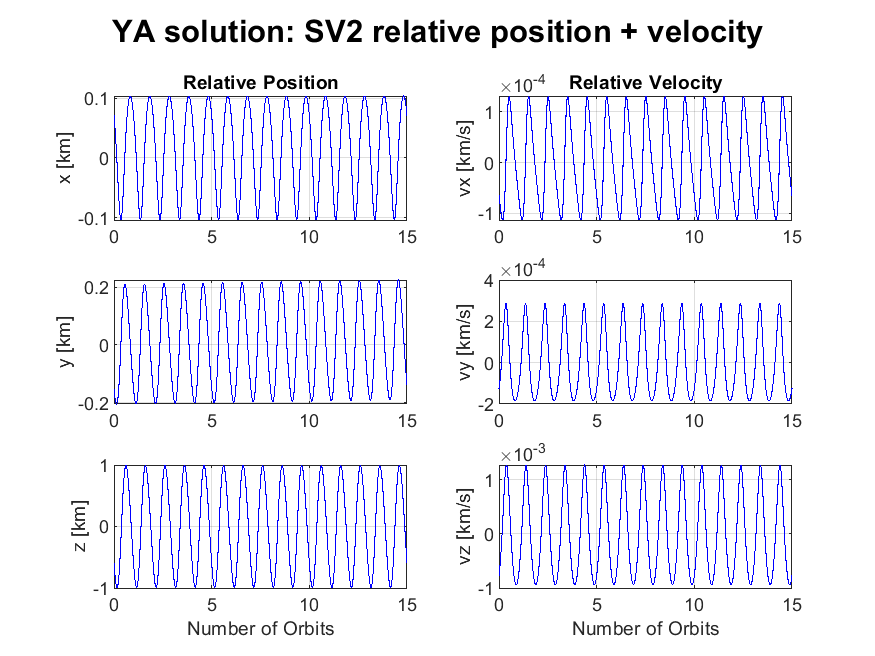
\includegraphics[width=0.7\linewidth]{sim/figures/PS3/YA_pos_vel_SV2.png}
    \caption{YA solution: 3D components of SV2 relative position and velocity}
    \label{fig:YA_sol_3D_comp_SV2}
\end{figure}
\begin{figure}[H]
    \centering
    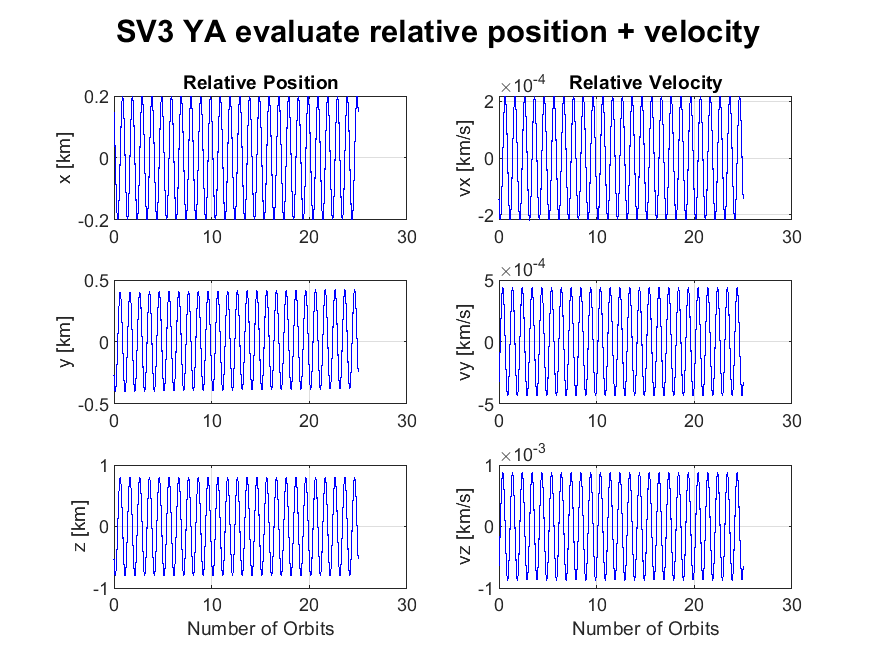
\includegraphics[width=0.7\linewidth]{sim/figures/PS3/YA_pos_vel_SV3.png}
    \caption{YA solution: 3D components of SV3 relative position and velocity}
    \label{fig:YA_sol_3D_comp_SV3}
\end{figure}
\begin{figure}[H]
    \centering
    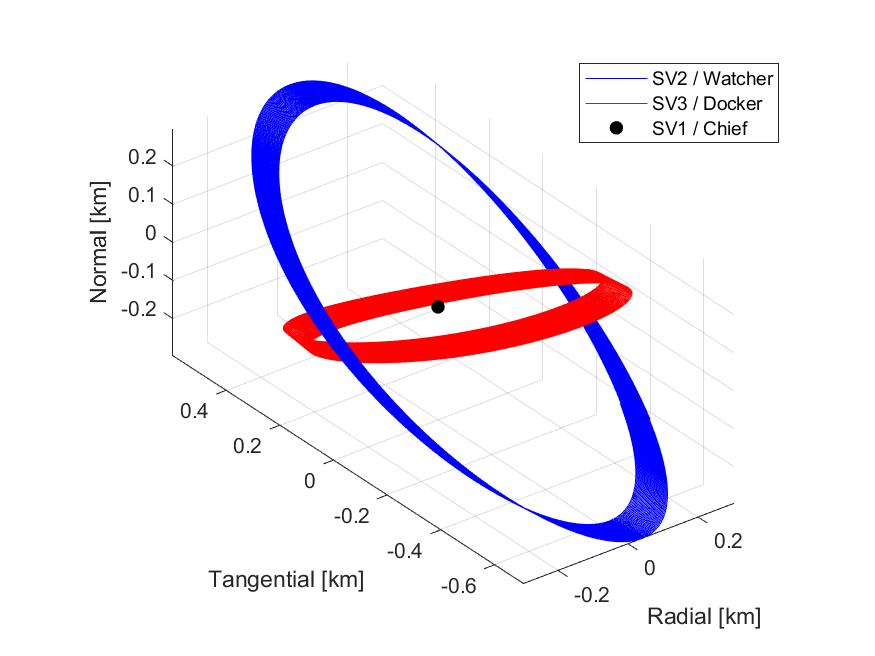
\includegraphics[width=0.7\linewidth]{sim/figures/PS3/YA_sol_3D_orbits.png}
    \caption{YA Solution: 3D Orbits of SV2 and SV3}
    \label{fig:YA_sol_3D_orbits}
\end{figure}
\begin{figure}[H]
    \centering
    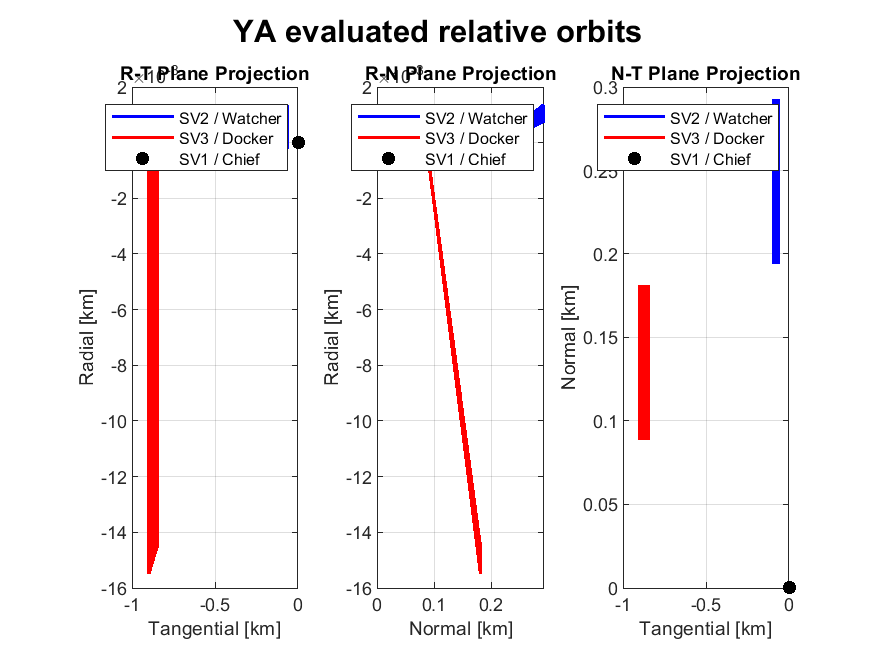
\includegraphics[width=0.7\linewidth]{sim/figures/PS3/RTN_projections_YA.png}
    \caption{YA Solution: Relative orbit RTN projections}
    \label{fig:YA_sol_RTN}
\end{figure}

\subsubsection{Analysis of YA Solution Results}\label{sec:YA_sol_analysis}
These results line up with our expectations given the chosen initial conditions and integration constants. We chose to align the relative eccentricity and inclination vectors to create ellipses in the RT plane that do not intersect with the chief (i.e. passive safety). These ellipses also do not intersect with the chief in the RN plane. 

As explained by Willis, the 2-by-1 ellipse in the RT plane is dictated by the magnitude and phase of the K3 and K2 integration constants. This aligns with our integration constants have larger magnitudes in K2, K3, and K5 for both SV1 and SV2. Specifically the radial axis corresponds to K3, while the tangential axis corresponds to K2. While the Figures are compressed, the 2-by-1 ellipse is actually oriented in the horizontal direction with the major axis in the tangential direction and the minor axis in the radial direction. This matches the bounding ellipse given by Willis. 

The relative motion is not fully bounded as expected from the energy matching condition. This is because the TH equations have a secular term in the tangential direction that is governed by the integration constant, $c_3$. Unless the initial relative position and velocity are set precisely to make $c_3$ equal to zero, there will be along-track drift. This drift could be mitigated by finding those initial conditions from the following expression:
\[
c_3 = k(f(0)) y'(f(0)) + e \sin f(0) \left[ x'(f(0)) - y(f(0)) \right] + \left[ 2 + e \cos f(0) \right] x(f(0)) = 0
\]

\subsubsection{Quasi-Nonsingular Relative Orbit Elements}
For the eccentric orbit case, we will use the same quasi-nonsingular ROE as outlined in Table \ref{tab:relative_oe_hcw}.

\subsubsection{Relative State Propagation Using Geometric Linear Mapping}
Another method for propagating the relative position and velocity is through geometric linear mapping with relative orbit elements. This method is described by Willis and is as follows \cite{willis2023analytical}.

The following expressions are defined:
\begin{align}
n &= \sqrt{\frac{\mu_{\text{earth}}}{a^3}}, \quad
e = \sqrt{e_x^2 + e_y^2}, \quad
\eta = \sqrt{1 - e^2} \\
\text{ROE}_{\text{init}} &= 
\begin{bmatrix}
\delta a \\ \delta \lambda \\ \delta e_x \\ \delta e_y \\ \delta i_x \\ \delta i_y
\end{bmatrix}
\end{align}

Then for each time step ($t$) in the time array ($t_i$), the following expressions are computed:
\begin{align}
M &= (M_{\text{init}}) + n t_i \\
E &= \texttt{Newton\_Raphson}(M, e, 10^{-5}) \\
f &= 2 \tan^{-1} \left( \sqrt{\frac{1 + e}{1 - e}} \tan\left( \frac{E}{2} \right) \right) \\
f &= f \mod 2\pi \\
u &= \omega + f \\
k &= 1 + e_x \cos u + e_y \sin u \\
k' &= -e_x \sin u + e_y \cos u
\end{align}

Then the $A$ matrix is computed:
\begin{align}
A = 
\begin{bmatrix}
a \eta^2 I_{3 \times 3} & 0 \\
0 & \dfrac{a n}{\eta} I_{3 \times 3}
\end{bmatrix}
\end{align}

And the $B$ matrix is computed:
\begin{align}
b_{x1} &= \frac{1}{k} + \frac{3}{2}k' \left(\frac{n}{\eta^3}\right)t &
b_{x2} &= -\frac{k'}{\eta^3} \\
b_{x3} &= \frac{1}{\eta^3}\left(\frac{e_x(k - 1)}{1 + \eta} - \cos u\right) &
b_{x4} &= \frac{1}{\eta^3}\left(\frac{e_y(k - 1)}{1 + \eta} - \sin u\right) \\
b_{x6} &= \frac{k'}{\eta^3} \cot i \\
b_{y1} &= -\frac{3}{2}k \left(\frac{n}{\eta^3}\right)t &
b_{y2} &= \frac{k}{\eta^3} \\
b_{y3} &= \frac{1}{\eta^2}\left[(1 + \frac{1}{k})\sin u + \frac{e_y}{k} + \frac{k}{\eta}\left(\frac{e_y}{1 + \eta}\right)\right] \\
b_{y4} &= -\frac{1}{\eta^2}\left[(1 + \frac{1}{k})\cos u + \frac{e_x}{k} + \frac{k}{\eta}\left(\frac{e_x}{1 + \eta}\right)\right] \\
b_{y6} &= \left(\frac{1}{k} - \frac{k}{\eta^3} \right) \cot i \\
b_{z5} &= \frac{1}{k} \sin u, \quad
b_{z6} = -\frac{1}{k} \cos u
\end{align}
\begin{align}
\dot{b}_{x1} &= \frac{k'}{2} + \frac{3}{2}k^2(1 - k)\left(\frac{n}{\eta^3}\right)t \\
\dot{b}_{x2} &= \frac{k^2}{\eta^3}(k - 1), \quad
\dot{b}_{x3} = \frac{k^2}{\eta^3}\left[\eta \sin u + e_y \left( \frac{k - 1}{1 + \eta} \right)\right] \\
\dot{b}_{x4} &= -\frac{k^2}{\eta^3}\left[\eta \cos u + e_x \left( \frac{k - 1}{1 + \eta} \right)\right], \quad
\dot{b}_{x6} = -\frac{k^2}{\eta^3}(k - 1)\cot i
\end{align}
\begin{align}
\dot{b}_{y1} &= -\frac{3}{2}k\left[1 + kk'\left(\frac{n}{\eta^3}\right)t\right] \\
\dot{b}_{y2} &= \frac{k^2}{\eta^3}k', \quad
\dot{b}_{y3} = \left[1 + \frac{k^2}{\eta^3}\right]\cos u + e_x\left(\frac{k}{\eta^2}\left[1 + \frac{k}{\eta}\left(\frac{1 - k}{1 + \eta}\right)\right]\right) \\
\dot{b}_{y4} &= \left[1 + \frac{k^2}{\eta^3}\right]\sin u + e_y\left(\frac{k}{\eta^2}\left[1 + \frac{k}{\eta}\left(\frac{1 - k}{1 + \eta}\right)\right]\right) \\
\dot{b}_{y6} &= -\left[1 + \frac{k^2}{\eta^3}\right]k'\cot i \\
\dot{b}_{z5} &= \cos u + e_x, \quad
\dot{b}_{z6} = \sin u + e_y
\end{align}

\[
B =
\begin{bmatrix}
b_{x1} & b_{x2} & b_{x3} & b_{x4} & 0     & b_{x6} \\
b_{y1} & b_{y2} & b_{y3} & b_{y4} & 0     & b_{y6} \\
0      & 0      & 0      & 0      & b_{z5} & b_{z6} \\
\dot{b}_{x1} & \dot{b}_{x2} & \dot{b}_{x3} & \dot{b}_{x4} & 0 & \dot{b}_{x6} \\
\dot{b}_{y1} & \dot{b}_{y2} & \dot{b}_{y3} & \dot{b}_{y4} & 0 & \dot{b}_{y6} \\
0      & 0      & 0      & 0      & \dot{b}_{z5} & \dot{b}_{z6}
\end{bmatrix}
\]

Finally, the relative state (position and velocity) is computed at each time step:
\begin{align}
\texttt{relative states}(i, :) &= (A B \cdot \text{ROE}_{\text{init}})^T
\end{align}

The resulting relative position and velocity 3D components of SV2 and SV3 are shown in Figures \ref{fig:YA_map_3D_comp_SV2} and \ref{fig:YA_map_3D_comp_SV3} respectively. Both SV2 and SV3 orbits are plotted in 3D in Figure \ref{fig:YA_map_3D_orbits}. Finally, the RTN projections of the relative orbits are shown in Figure \ref{fig:YA_map_RTN}.

\begin{figure}[H]
    \centering
    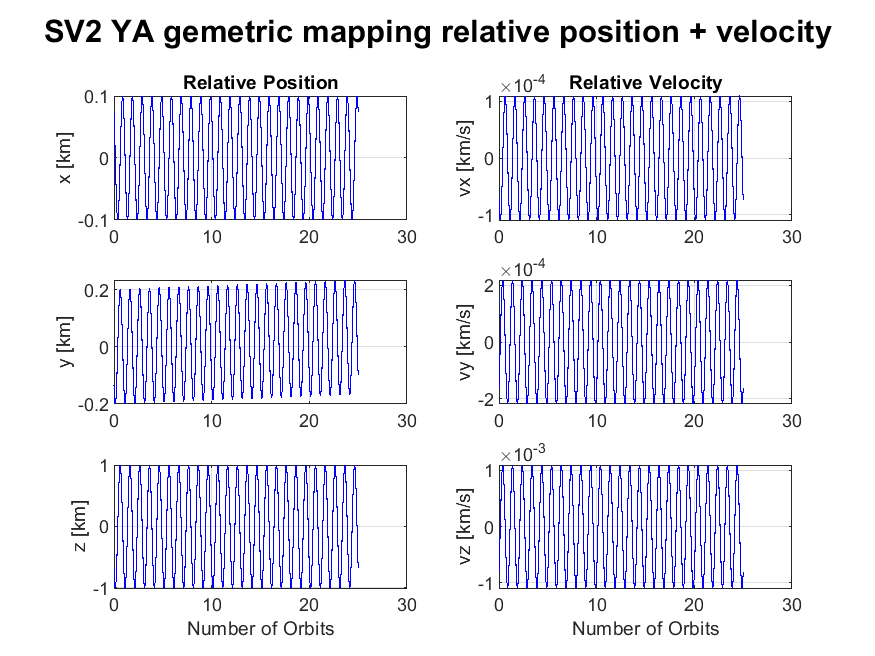
\includegraphics[width=0.7\linewidth]{sim/figures/PS3/YA_mapping_pos_vel_SV2.png}
    \caption{YA geometric linear mapping: 3D components of SV2 relative position and velocity}
    \label{fig:YA_map_3D_comp_SV2}
\end{figure}
\begin{figure}[H]
    \centering
    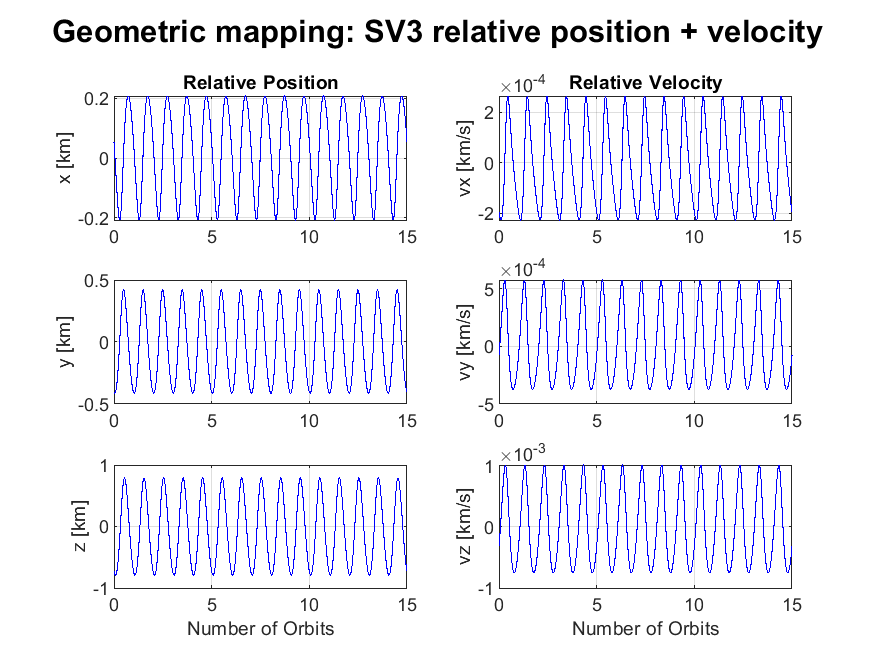
\includegraphics[width=0.7\linewidth]{sim/figures/PS3/YA_mapping_pos_vel_SV3.png}
    \caption{YA geometric linear mapping: 3D components of SV3 relative position and velocity}
    \label{fig:YA_map_3D_comp_SV3}
\end{figure}
\begin{figure}[H]
    \centering
    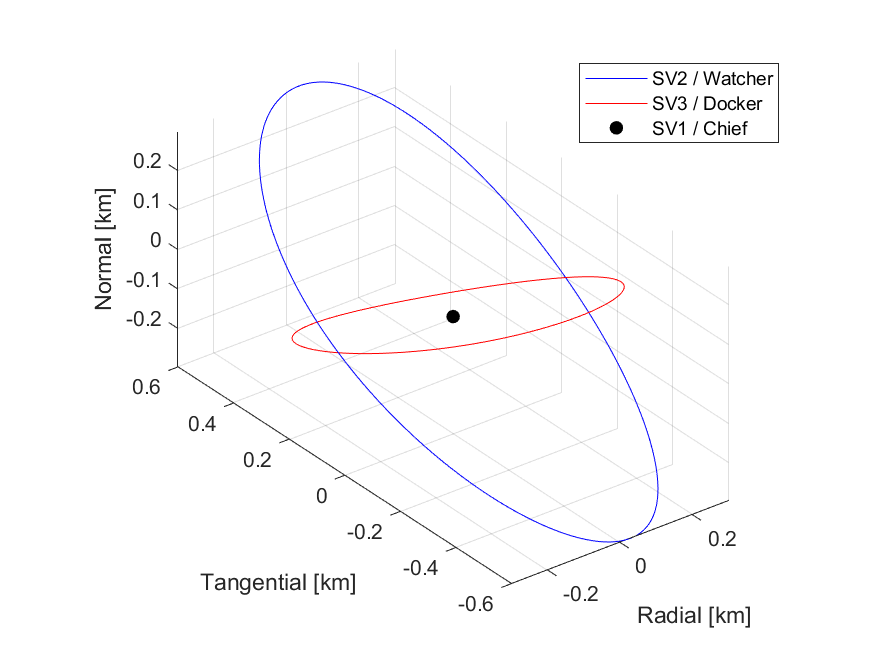
\includegraphics[width=0.7\linewidth]{sim/figures/PS3/YA_mapping_3D_orbits.png}
    \caption{YA geometric linear mapping: 3D Orbits of SV2 and SV3}
    \label{fig:YA_map_3D_orbits}
\end{figure}
\begin{figure}[H]
    \centering
    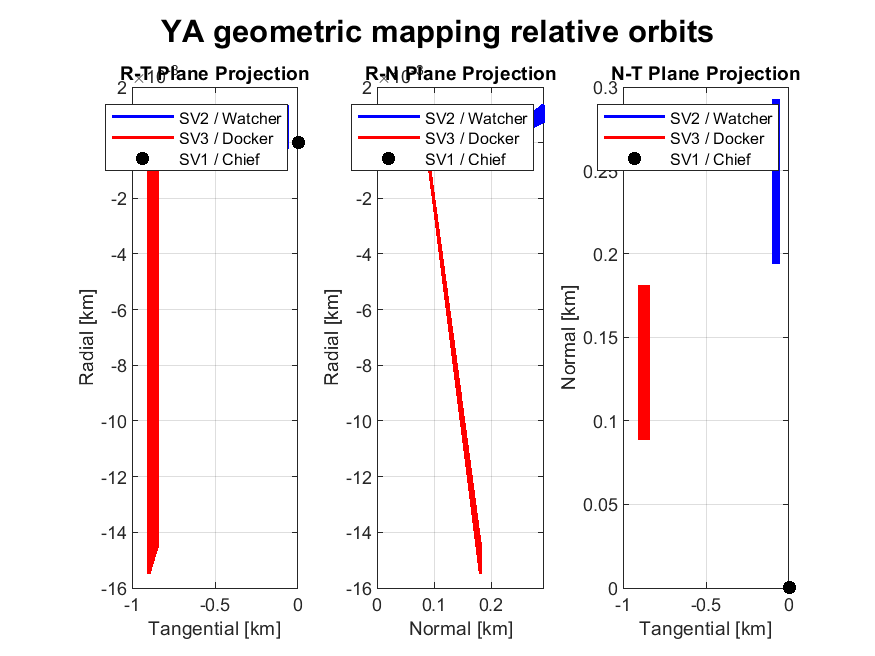
\includegraphics[width=0.7\linewidth]{sim/figures/PS3/RTN_projections_YA_mapping.png}
    \caption{YA geometric linear mapping: Relative orbit RTN projections}
    \label{fig:YA_map_RTN}
\end{figure}

\subsubsection{Analysis of Geometric Linear Mapping Results}\label{sec:geom_mapping_analysis}
The results from geometric linear mapping are as expected, because there are close to those from the YA solution but slightly different. Specifically, the ellipses are skewed differently and have different thicknesses in the tangential direction. This is expected because, as explained by Willis, geometric linear mapping is an approximation of the transformation from ROE to position and velocity vectors \cite{willis2023analytical}. The ROEs can be related to the position and velocity vecotrs of the chief and deputy spacecraft through the geometry of Keplerian orbits. But this is still an approximation and not a solution to the TH equations, like the previous method was. 

The unscaled ROE can be found by dividing the original ROE given in Table \ref{tab:relative_oe_hcw} by the chief's semi-major axis. They are computed for SV2 and SV3 to be:
\[
\text{ROE}_{\text{SV2}} = 
\begin{bmatrix}
\delta a \\ \delta \lambda \\ \delta e_x \\ \delta e_y \\ \delta i_x \\ \delta i_y
\end{bmatrix} =
\begin{bmatrix}
0 \\
0 \\
0 \\
0.4320 \times 10^{-4} \\
0 \\
0.4320 \times 10^{-4}
\end{bmatrix}
\]
\[
\text{ROE}_{\text{SV3}} = 
\begin{bmatrix}
\delta a \\ \delta \lambda \\ \delta e_x \\ \delta e_y \\ \delta i_x \\ \delta i_y
\end{bmatrix} =
\begin{bmatrix}
0 \\
0 \\
0 \\
0.3600 \times 10^{-4} \\
0 \\
-0.3600 \times 10^{-4}
\end{bmatrix}
\]

These match up with the integration constants computed before. Specifically, for both SV2 and SV3, approximately $K_3$ = $\delta e_y$ and $K_5$ = $\delta i_y$. Since there is is very little eccentricity in the x-direction, these quantities represent the relative eccentricity and inclination magnitudes. Thus $K_3$ corresponds to the relative eccentricity, while $K_5$ corresponds to the relative inclination of the deputy spacecraft. 


\subsubsection{Comparison of Errors from Different Propagation Methods}
Now we can compare YA solution and geometric mapping to the true relative position and velocity given by numerical propagation of the nonlinear equations (Fundamental Equations of Relative Motion or FERM) as outlined in Section \ref{sec:nonlinear_rel_eom}. Note that the YA solution method is referred to as "YA Dif. Eq." and the geometric mapping method is referred to as "YA Mapping" in the Figures. 

\begin{figure}[H]
    \centering
    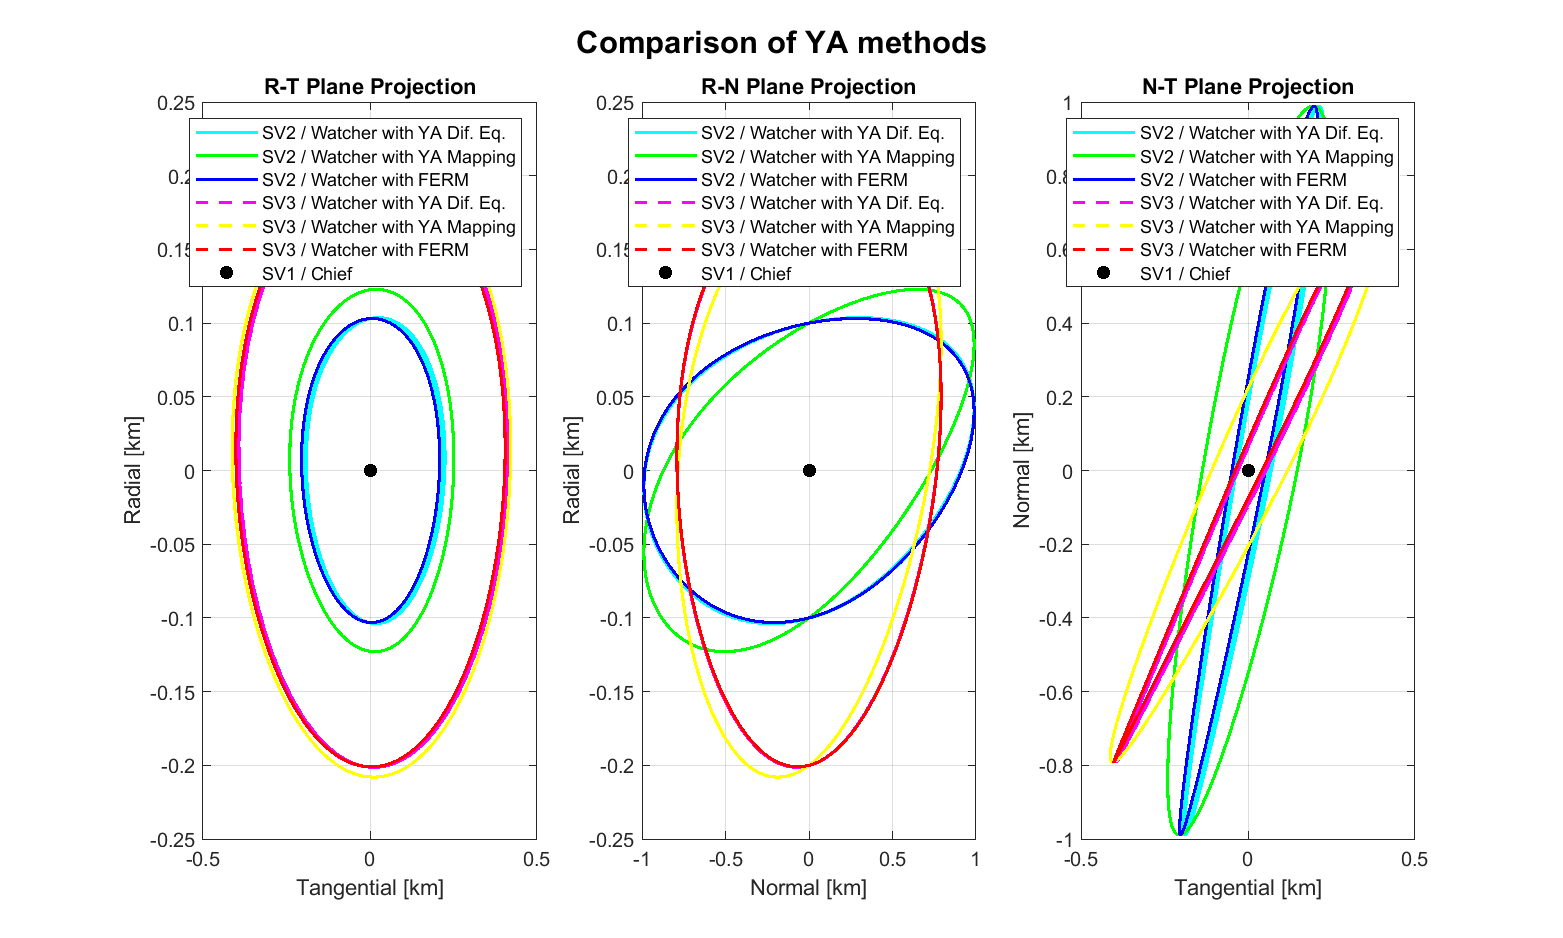
\includegraphics[width=0.7\linewidth]{sim/figures/PS3/RTN_projections_YA_comparison.png}
    \caption{RTN projections of YA Solution, Geometric Mapping, and FERM}
    \label{fig:RTN_YA_comp}
\end{figure}
\begin{figure}[H]
    \centering
    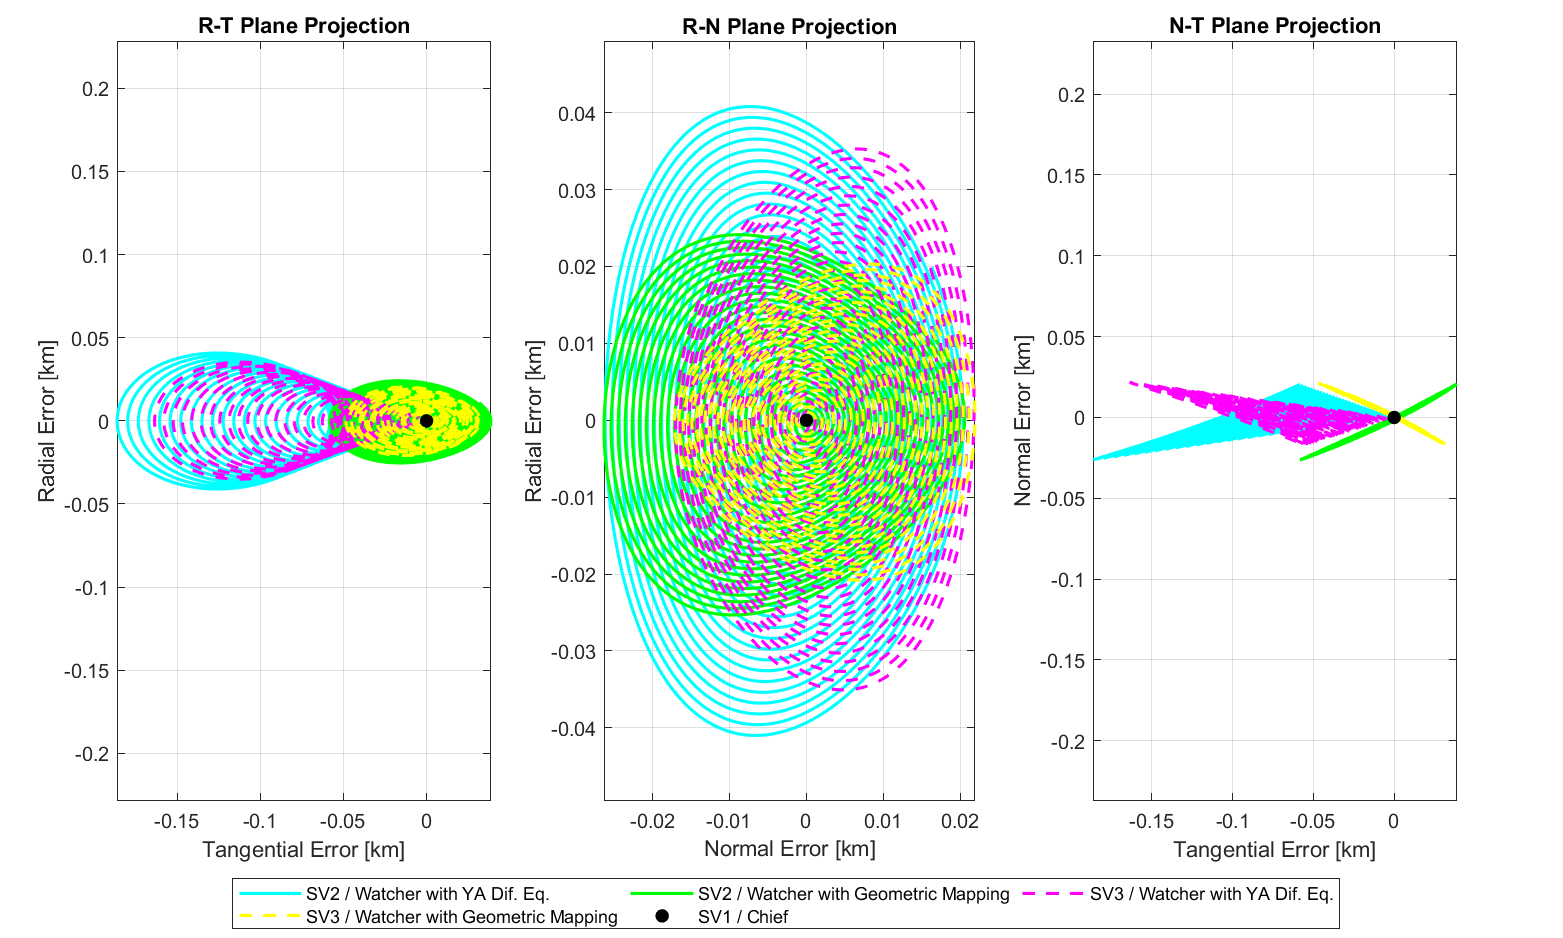
\includegraphics[width=0.7\linewidth]{sim/figures/PS3/RTN_error_projections_YA_comparison.png}
    \caption{RTN projections of error between YA Solution, Geometric Mapping and FERM}
    \label{fig:RTN_error_comp}
\end{figure}
\begin{figure}[H]
    \centering
    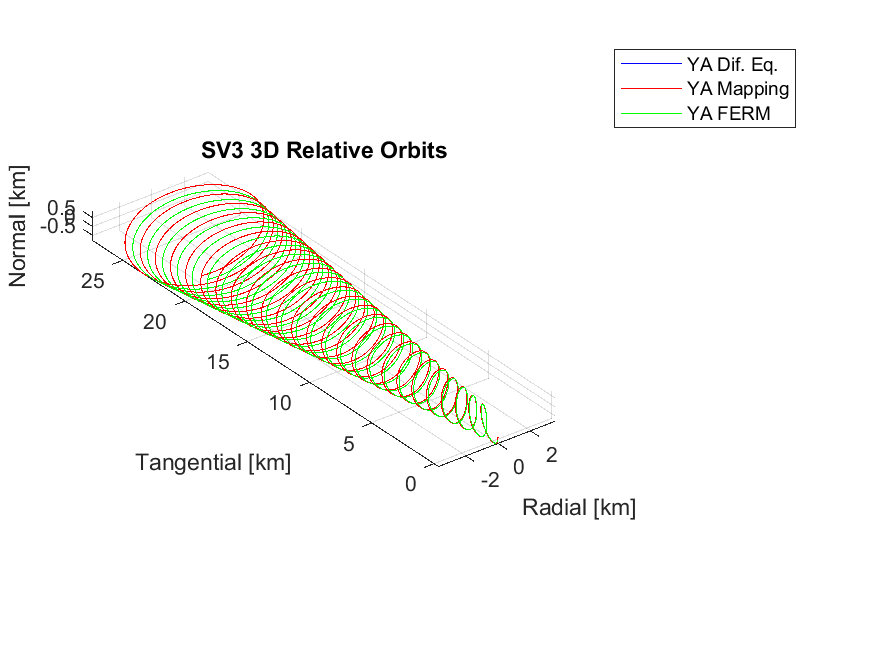
\includegraphics[width=0.7\linewidth]{sim/figures/PS3/3D_YA_comparison.png}
    \caption{3D orbits propagated from YA Solution, Geometric Mapping and FERM}
    \label{fig:3D_orbits_comp}
\end{figure}

These plots show that the YA solution of the differential equation is more accurate than geometric mapping, as the YA solution is much closer to the true motion. While geometric mapping is close to the true motion, it exhibits significant errors. This is because, as discussed in Section \ref{sec:geom_mapping_analysis}, geometric mapping is a linear approximation relating the ROEs to the integration constants and thus to the relative motion. On the other hand, the YA solution is intrinsic to the YA model as the relative motion is inherently linked to the integration constants. 

\subsubsection{Repeating with Difference in Semi-Major Axis}
Now, following the same procedure outlined above, we can adjust the initial conditions to investigate the behavior when there is a difference in semi-major axis between the deputy and the chief. We chose to apply the following conditions, while maintaining all other initial conditions the same. 

\begin{align*}
\delta a_{\text{SV2, init}} &= 200 \ \text{m} \\
\delta a_{\text{SV3, init}} &= -100 \ \text{m}
\end{align*}

These were chosen to illustrate how SV2's higher orbit and SV3's lower orbit would affect the along-track drift. Since both deputy orbits now have different semi-major axes than the chief, we expect to see along-track drift. Specifically, we expect to see the along-track drift go in opposite directions: for the higher orbit we expect the deputy to drift behind the chief, while for the lower orbit we expect the deputy to drift ahead of the chief. For the magnitude of the drift, we expect significant drift since the original initial conditions already had drift with the energy matching condition and now the energy matching condition is taken away. The drift dependent upon the $c_3$ integration constant discussed in Section \ref{sec:YA_sol_analysis}. Given the initial conditions and an initial separation of about 0.6 km between the spacecraft, we expect the drift to be a few km per orbit. 

Figure \ref{fig:RTN_comp_2} shows the new RTN projections of all YA methods now with the introduced semi-major axis separation. Figure \ref{fig:RTN_error_comp_2} shows the new RTN error projections of all YA methods. Figure \ref{fig:3D_orbits_YA_comp_2} shows the 3D orbits of all YA methods. 

\begin{figure}[H]
    \centering
    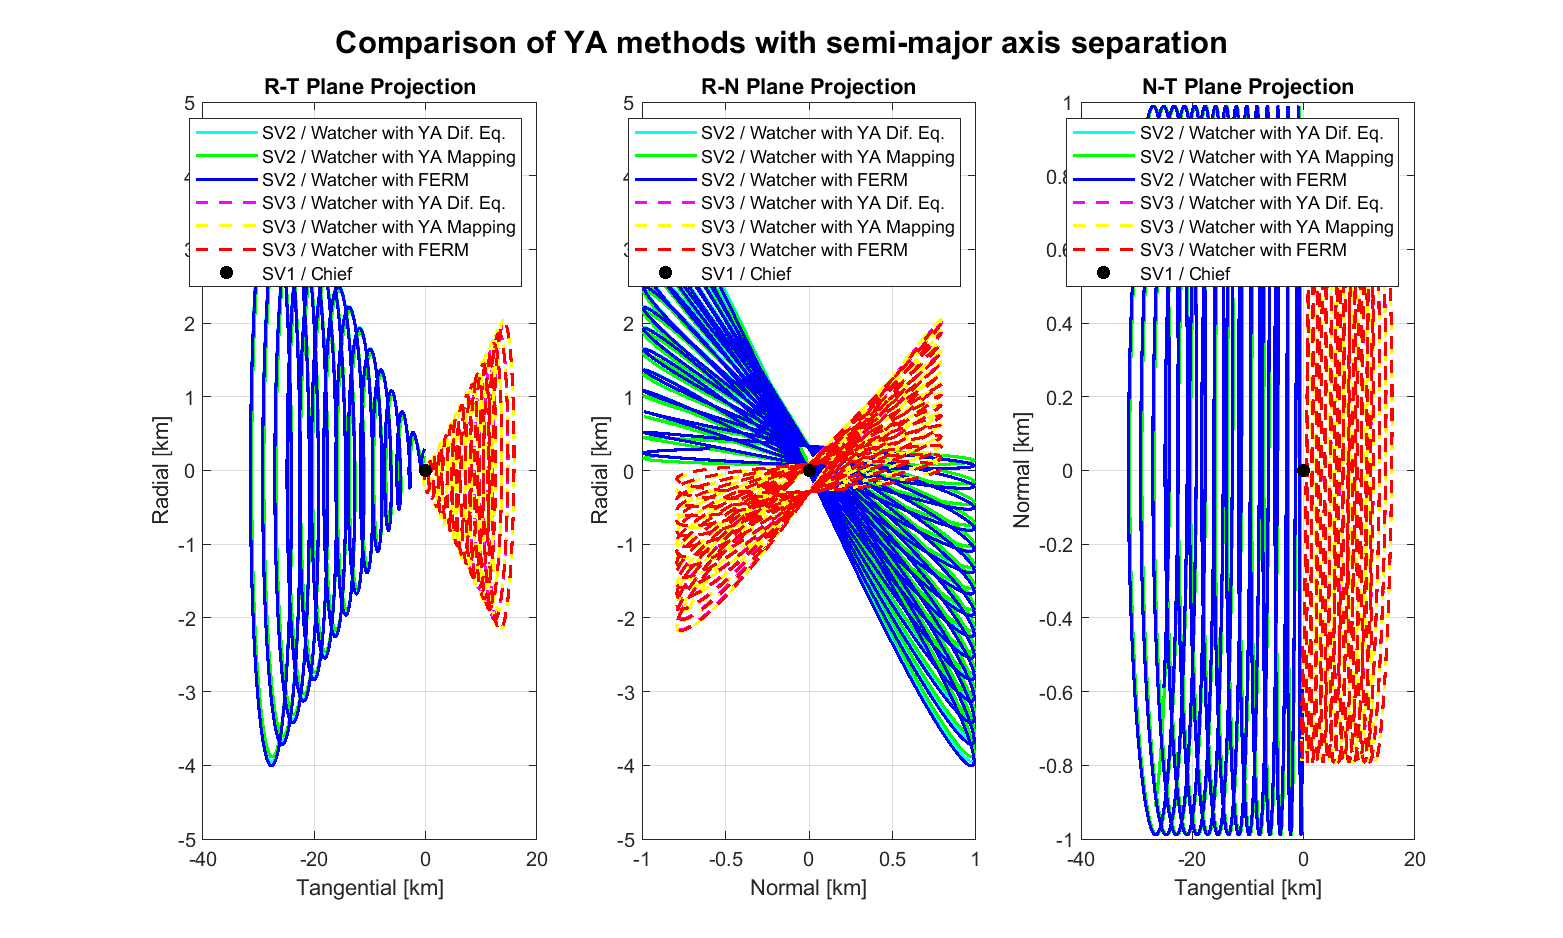
\includegraphics[width=0.7\linewidth]{sim/figures/PS3/RTN_projections_YA_comparison_2.png}
    \caption{RTN projections of YA methods with semi-major axis separation}
    \label{fig:RTN_comp_2}
\end{figure}
\begin{figure}[H]
    \centering
    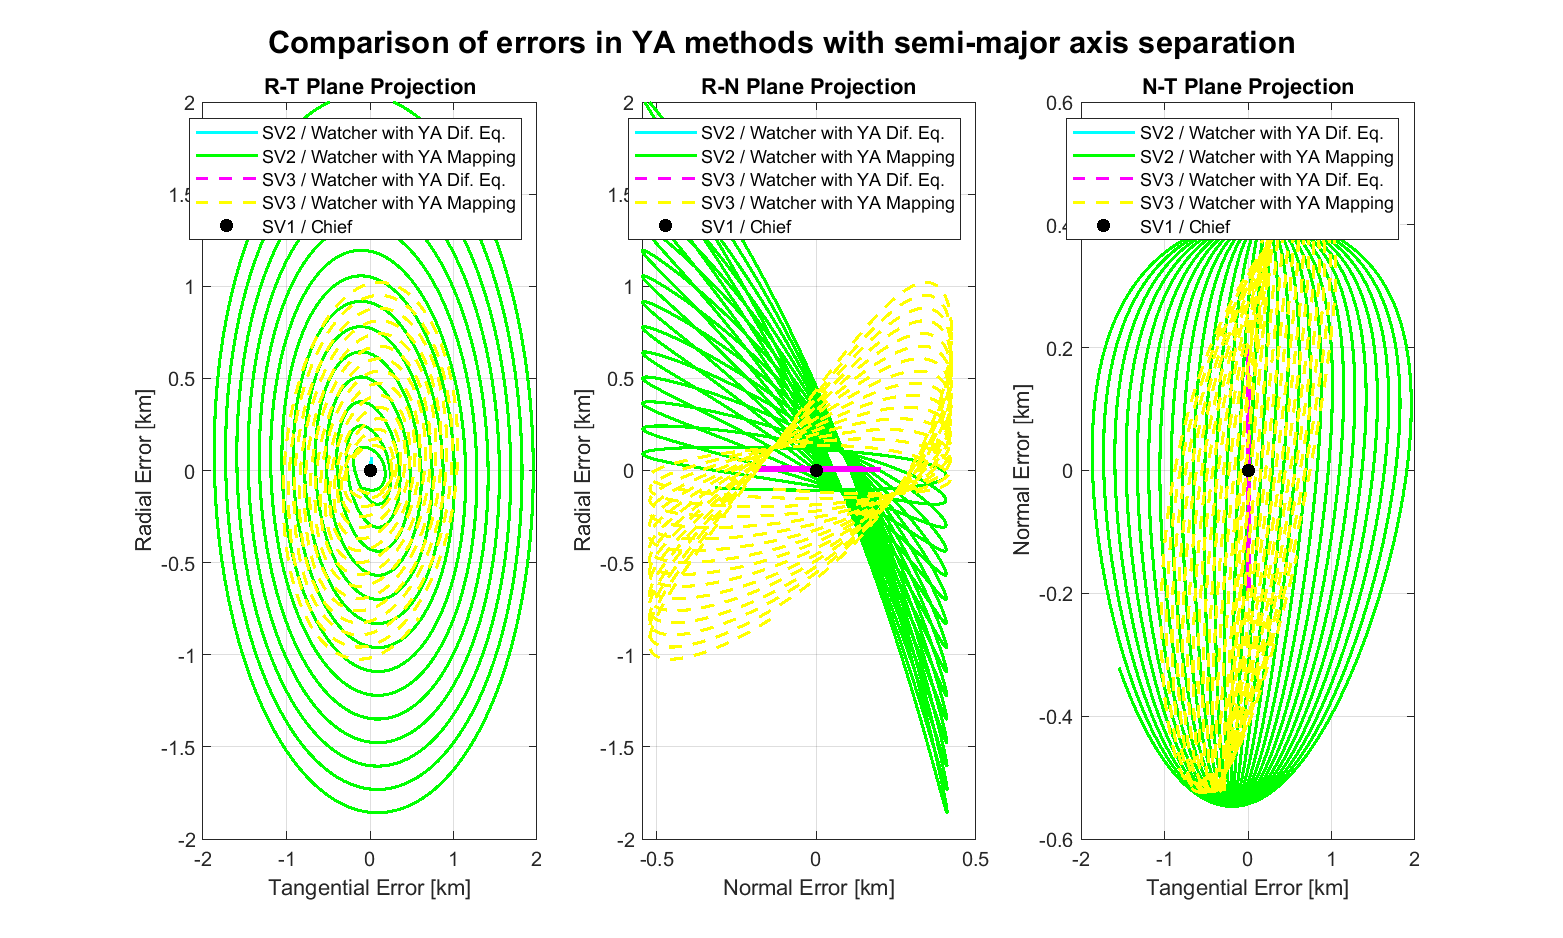
\includegraphics[width=0.7\linewidth]{sim/figures/PS3/RTN_error_projections_YA_comparison_2.png}
    \caption{RTN error projections of YA methods with semi-major axis separation}
    \label{fig:RTN_error_comp_2}
\end{figure}
\begin{figure}[H]
    \centering
    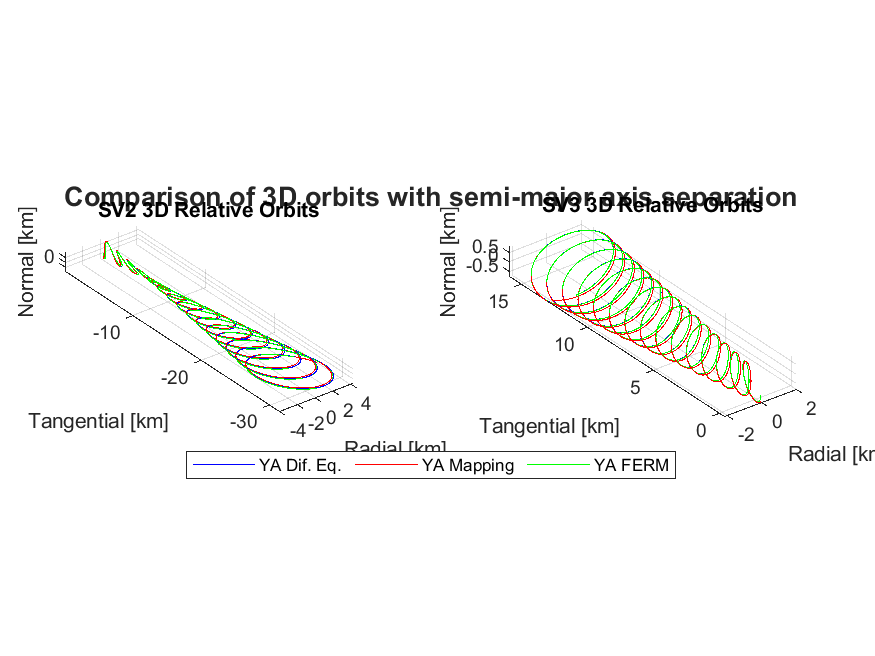
\includegraphics[width=0.7\linewidth]{sim/figures/PS3/3D_YA_comparison_2.png}
    \caption{3D orbits of YA methods with semi-major axis separation}
    \label{fig:3D_orbits_YA_comp_2}
\end{figure}

As expected, there is significant drift arising from the differences in semi-major axis. Tangentially, SV2 drifts behind the chief since SV2 is above the chief and has a longer orbital period, while SV3 drifts ahead of the chief since SV3 is below the chief and thus has a shorter orbital period. There is also a radial drift which causes the deputy orbits to rotate about the tangential axis. This is due to the coupled nature of the tangential and radial components in the TH equations. The normal components are unaffected as out-of-plane behavior is decoupled from in-plane behavior. As before, the YA solution of the differential equation is much more accurate than the geometric linear mapping, which has significant and growing errors. The 3D orbits are as expected as they loop around the chief orbit with drift in tangential and radial directions.

\subsubsection{Repeating with Highly Eccentric Chief Orbit}
Now, following the same procedure outlined above, we can adjust the initial conditions to investigate the behavior when there is a highly eccentric chief orbit. We chose to apply the following condition, while maintaining all other original initial conditions the same. 
\begin{align*}
e_{SV1} &= 0.55 \\
\end{align*}
Figure \ref{fig:RTN_comp_3} shows the new RTN projections of all YA methods now with the introduced semi-major axis separation. Figure \ref{fig:RTN_error_comp_3} shows the new RTN error projections of all YA methods. Figure \ref{fig:3D_orbits_YA_comp_3} shows the 3D orbits of all YA methods. 

\begin{figure}[H]
    \centering
    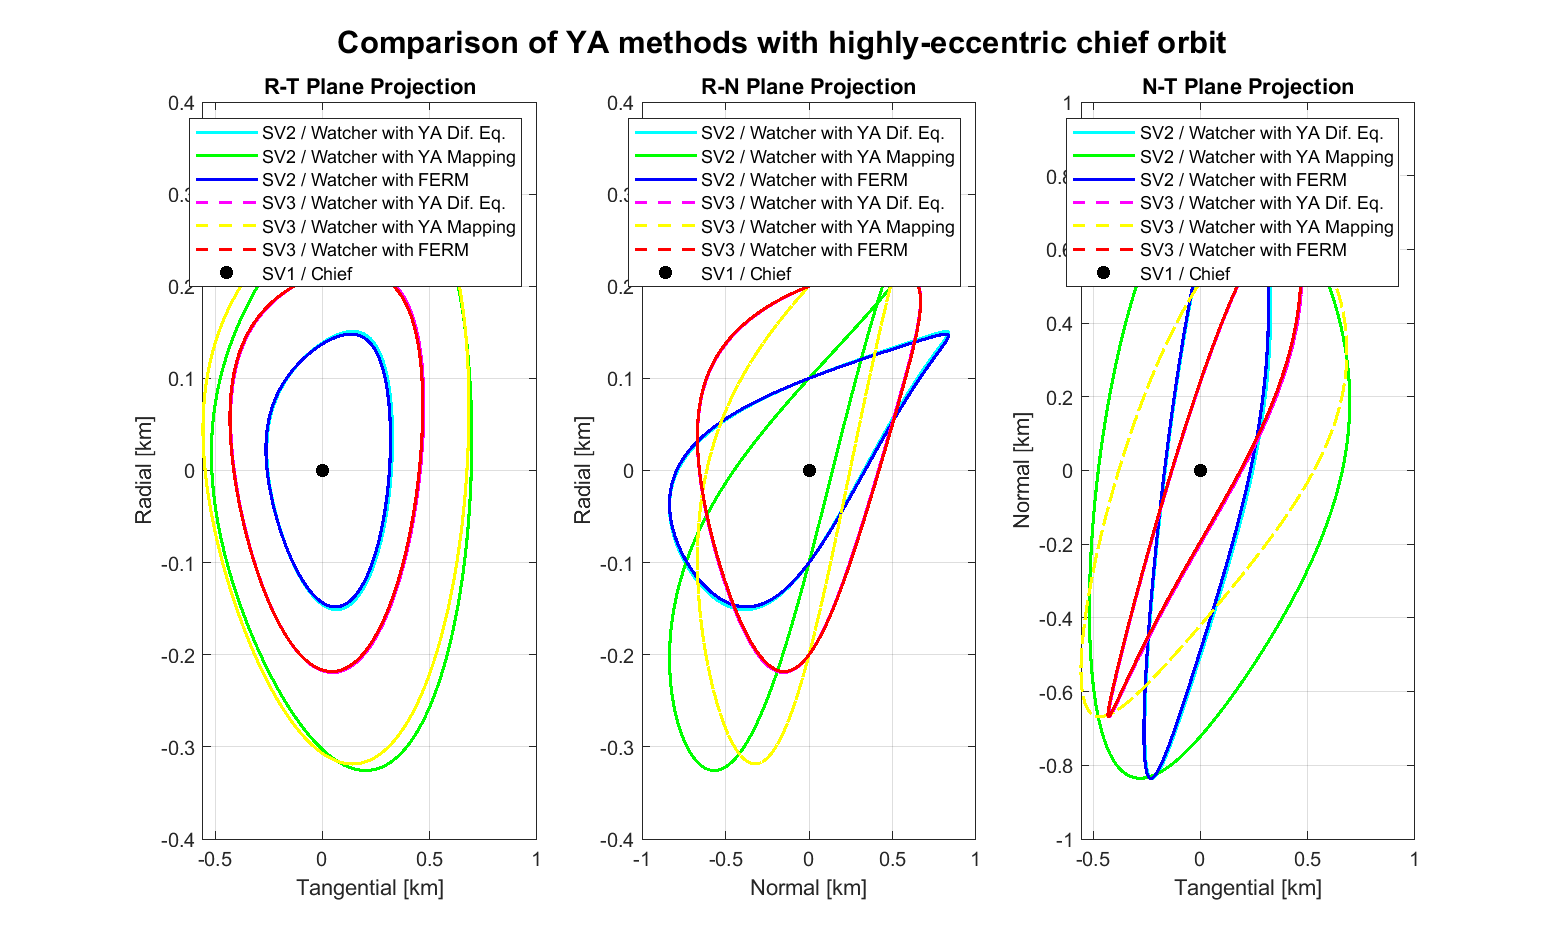
\includegraphics[width=0.7\linewidth]{sim/figures/PS3/RTN_projections_YA_comparison_3.png}
    \caption{RTN projections of YA methods with highly-eccentric chief orbit}
    \label{fig:RTN_comp_3}
\end{figure}
\begin{figure}[H]
    \centering
    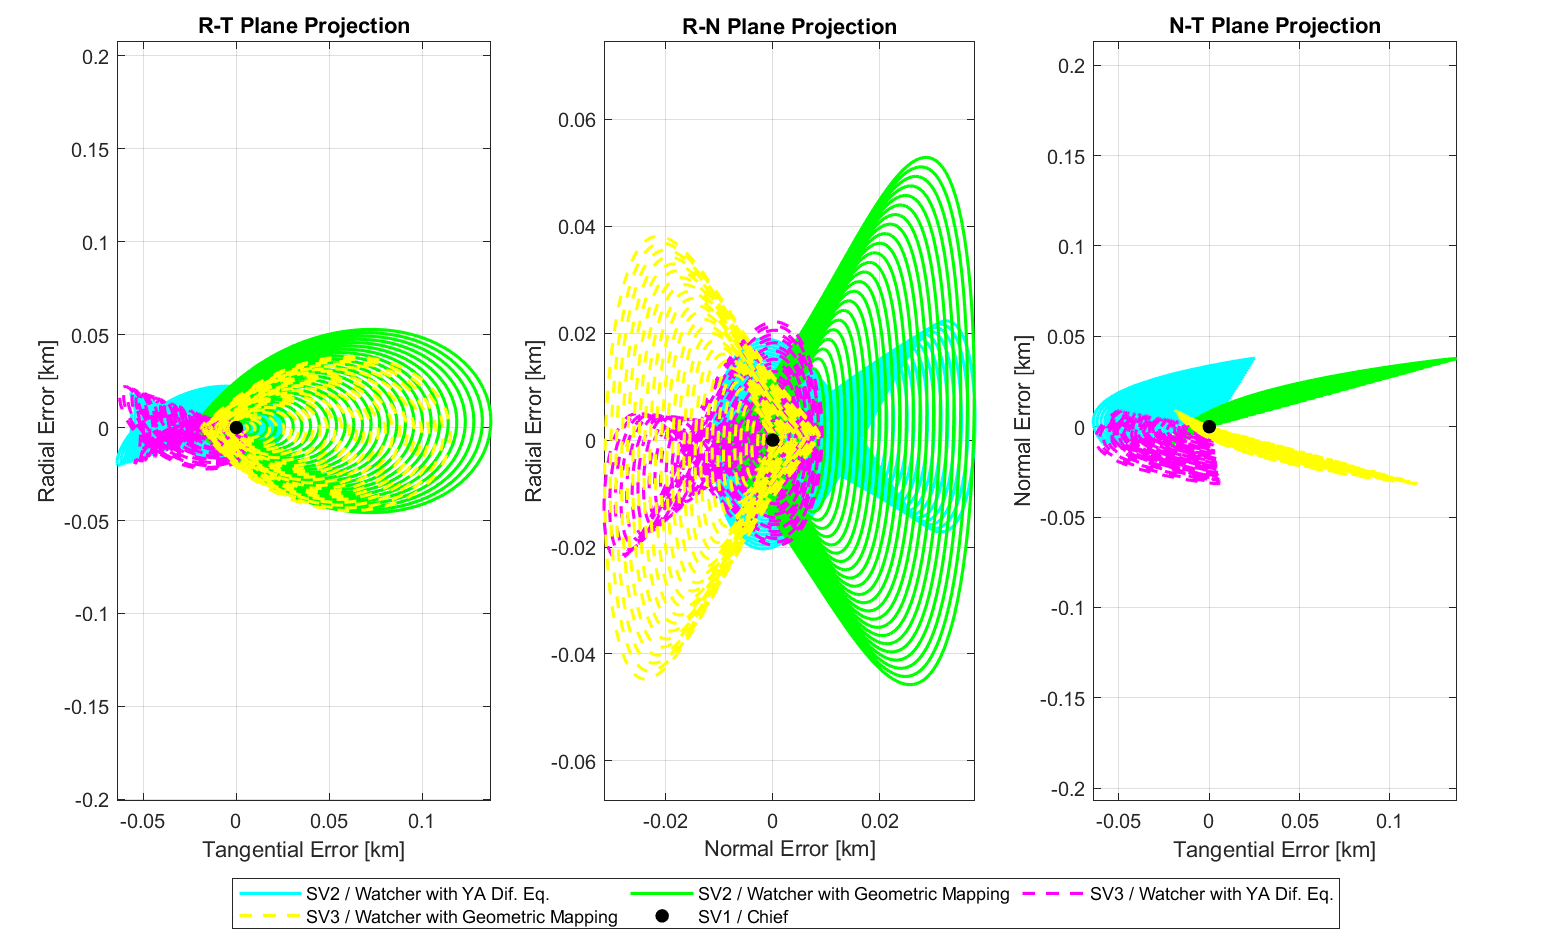
\includegraphics[width=0.7\linewidth]{sim/figures/PS3/RTN_error_projections_YA_comparison_3.png}
    \caption{RTN error projections of YA methods with highly-eccentric chief orbit}
    \label{fig:RTN_error_comp_3}
\end{figure}
\begin{figure}[H]
    \centering
    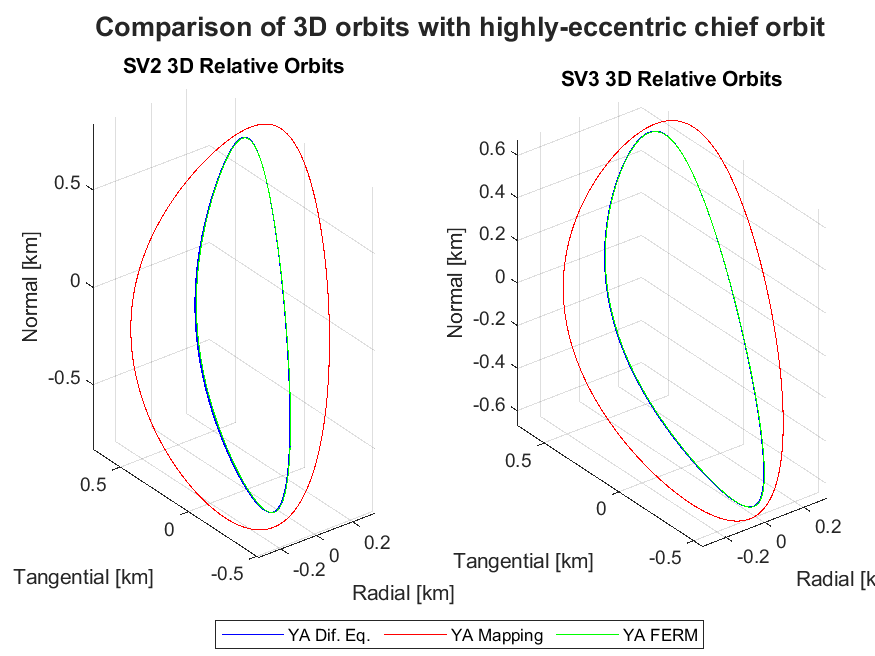
\includegraphics[width=0.7\linewidth]{sim/figures/PS3/3D_YA_comparison_3.png}
    \caption{3D orbits of YA methods with highly-eccentric chief orbit}
    \label{fig:3D_orbits_YA_comp_3}
\end{figure}

As expected, the high eccentricity skews relative motion away from the normal 2:1 ellipses. As Willis explains the relative position in the RT plane is bounded by two ellipses which rely on the eccentricity of the chief's orbit \cite{willis2023analytical}. As eccentricity is increased these ellipses are stretched out or skewed, which leads to the behavior found here. Again, the geometric mapping method exhibits much larger error than the solution of the differential equation. 